%!TEX root = Thesis.tex

\chapter{Experimental}
\label{ch:expt}

\section{General Procedures}
\label{section:generalprocedures}

\setlength{\emergencystretch}{2pt}

\begin{sloppypar}
All reactions and manipulation of products and reagents were carried out under an inert nitrogen or argon atmosphere using standard Schlenk line techniques unless stated otherwise.  All reactions using silver compounds were performed in the dark.  Unless otherwise stated the starting materials used in this work were obtained from Sigma-Aldrich, Merck Chemical Companies, Thermo Fisher Scientific, and BOC Industrial Gases, and used without further purification.  Analytical grade reagents and high purity solvents were degassed and purged with argon before use, and dried over molecular sieves.  Diethyl ether and tetrahydrofuran were distilled under an argon atmosphere from sodium benzophenone ketyl immediately prior to use.  
1,3,5-tri\-aza-7-phos\-pha\-adamantane,\cite{Daigle1998a} 
\emph{sec}-Butyllithium,\cite{Dieter2001} 
2,8-di\-methyl\-phenoxathiin,\cite{Suter1938} 
10,10-dimethyl\-phenoxasilin,\cite{Kranenburg1995} 
\ce{CH2(SO2CF3)2},\cite{Koshar1973} 
[Pt(nb\ce{)3}],\cite{Vaughan2011}
\ce{[Rh(coe)2Cl]2},\cite{Giordano1979}
 [Pt(\ce{C2H4)3}],\cite{Spencer1979} 
 [Pt\ce{Cl2(NCMe)2}],\cite{Hartley1979} 
[Pt(cod\ce{)2}],\cite{Crascall1990} 
[Pt(\ce{C6H10)Cl2]},\cite{Jensen1953} 
[Pt\ce{Cl2(SEt2)2}],\cite{Albrecht2000} 
[Pt\ce{Cl2(^{t}BuCN)2}],\cite{Cramer1967}
[Pd(nb\ce{)3}]\cite{Green1977}, 
[Pt(\ce{C6H10)ClMe}],\cite{Bradthesis}
[Pd(cod)\ce{Cl2}],
and [Pt(\ce{C6H10)Me2]},\cite{Vaughan2011}
were prepared according to literature procedures.  
\end{sloppypar}

NMR spectra were recorded using a Varian Unity Inova 300 (300~MHz for \proton, 75~MHz for \carbon, 121~MHz for \phosphorus{} and 282~MHz for \fluorine), a Varian Unity Inova 500 (500~MHz for \proton{} and 125~MHz for \carbon), or a Varian DirectDrive 600 (600~MHz for \proton\ and 150~MHz for \carbon{}) spectrometer.   The 600~MHz instrument was equipped with a Varian inverse-detected triple-resonance HCN cold probe operating at 25~K.  All direct-detected \proton{} and \carbon{} chemical shifts were referenced to the residual solvent peak.\cite{Fulmer2010}  NMR samples were prepared under an inert nitrogen or argon atmosphere unless otherwise stated, using \ce{C6D6}, \ce{CDCl3}, \ce{CD2Cl2}, acetone-\ce{d6} and toluene-\ce{d8}.  Variable temperature NMR spectroscopy was carried out using a Varian Unity Inova 300~MHz NMR spectrometer.  Infrared spectra were recorded with a PerkinElmer Spectrum One FT-IR spectrophotometer in absorbance mode.  Electrospray ionisation mass spectrometry was recorded using an Agilent 6530 Q-TOF mass spectrometer, or performed by the Carbohydrate Chemistry Group at Industrial Research Limited, Lower Hutt, using a Waters Q-TOF Premier Tandem mass spectrometer.

Single crystal X-ray diffraction data was solved using the Superflip program\cite{Superflip} (except for [Ag(\tButhixantphos)Cl] which was solved using the SHELX program) and refined using the SHELX program\cite{Shelx} with OLEX2 (version 1.2.5)\cite{Olex2} as a front-end.  Unless stated otherwise the hydrogen atoms were placed in calculated positions.  Crystallographic data was collected by the X-ray Crystallography Laboratory at the University of Canterbury, using either a Bruker SMART APEX-II CCD diffractometer or an Agilent SuperNova (Dual Source) CCD diffractometer.  Data were reduced using Bruker SAINT or Agilent CrysAlisPro software.  Absorption correction was performed using SADABS or SCALE3 ABSPACK.  Theoretical calculations were performed using the Gaussian 09 Revision B.01 program\cite{Gaussian09, Gaussian09b} running on the Victoria University of Wellington School of Chemical and Physical Sciences Heisenberg cluster, consisting of sixteen processing nodes with two 2.53 GHz Xeon X3440 quad-core processors per node and 1 GB of memory per core.  All searches of the Cambridge Structural Databank used version 5.35 (November 2013).\cite{Allen2002} 

%\fixme this will need to be checked with Matthias after submission.

%\fixme{All reactions with silver were performed in tinfoil wrapped vessels to prevent degradation due to light}
%\fixme{In the case of a 1:1 CDCl3:CD2Cl2 solvent mixing being used for NMR the spectra were referenced to the CD2Cl2 residual solvent peak}
%\subsection*{Crystallography} 
%\label{subsec:X-ray}

%Diffraction data\footnote{Bruker {\scriptsize{SMART}} (Version 5.054), {\scriptsize{SADABS}} (Version 2.03), and {\scriptsize{SAINT}} (Version 6.02A), Bruker AXS Inc., Madison, Wisconsin, USA, 1997.} (see Tables \ref{tab:dataPN582}, \ref{tab:dataPdPNCl2}, \ref{tab:datanbagostic}, \ref{tab:datadimer} for details) were collected using Bruker CCD diffractometers with Mo K$\alpha$ radiation (0.71073~\AA) from fine-focus sealed tubes with graphite monochromators, using phi and omega scans.  Multi-scan absorption corrections were applied.  The structures were solved by direct methods and full-matrix least squares refinement,\footnote{G. M. Sheldrick, {\scriptsize{SHELX-97}}.  Programmes for the Solution and Refinement of Crystal Structures, 1997.} with anisotropic thermal parameters for all non-H atoms.\cite{Sheldrick}  Hydrogen atoms are in calculated positions and refined using a riding model with {\scriptsize{SHELXL}} defaults.  The agostic hydrogen atom in \ce{Pt-H-C} interaction was located and its position refined, and all relevant bond distances and angles were calculated using Mercury, version 1.4.2.  Molecular drawings were made using ORTEP3.\cite{ORTEP}

\section{Ligands and Non-Transition Metal Derivatives}
\label{section:experimental:ligands}

%\pagevalues

%%%%%
%S-tBu %
%%%%%
%\newpage{}
\subsection*{2,8-Dimethyl-4,6-bis(di-\emph{tert}-butylphosphino)phenoxathiin \\(\emph{t}-Bu-thixantphos)}

%\begin{structure}
%\begin{center}
%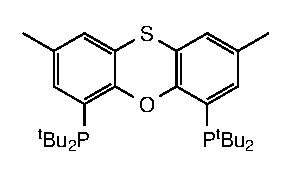
\includegraphics{../Structures/StBuligand.eps}
%\end{center}
%\end{structure}

\noindent{}\emph{sec}-Butyllithium (5.32 mL, 1.2 M in cyclohexane) was added dropwise to a stirred solution of 2,8-dimethylphenoxathiin (0.71 g, 3.1 mmol) and TMEDA (0.92 mL, 6.2 mmol) in diethyl ether (30 mL) at -78\degC{}.  The resulting yellow solution was allowed to warm to room temperature and stirred for a further 16 hours over which time a dark red colour developed.  The reaction was cooled to -78\degC{} and chlorodi-\emph{t}-butylphosphine (1.18 mL, 6.2 mmol) was added dropwise.  The reaction mixture was stirred for a further seven days resulting in a yellow solution with a white precipitate of lithium chloride.  The solvent was removed \emph{in vacuo} giving an orange oil.  This oil was dissolved in dichloromethane (25 mL) and washed with water (3 x 15 mL).  The organic layer was passed through a column of magnesium sulfate and solvent was removed \emph{in vacuo}.  The product was recrystallised from \emph{n}-propanol giving small white crystals (1.36 g, 85\%).  This compound can be handled in the air for short periods however, should be stored under an inert atmosphere.
\Phosphorusintro{CDCl3}
\NMRPsinglet{9.5}.
\Protonintro{500}{CDCl3}
\NMRsinglet{7.29}{\StBucH},
\NMRsinglet{6.88}{\StBuaH},
\NMRsinglet{2.25}{\StBugH},
\NMRmultiplet{1.22-1.24}{\StBuiH}.
\Carbonintro{125}{CDCl3}
\NMRPC{155.3}{vt}{13.0}{\StBueC},
\NMRsinglet{134.6}{\StBucC},
\NMRsinglet{131.9}{\StBubC},
\NMRcoupled{128.0}{dd}{22.5, 17.7}{\StBudC},
\NMRsinglet{127.4}{\StBuaC},
\NMRPC{120.1}{vt}{2.4}{\StBufC},
\NMRcoupled{32.9}{dd}{15.8, 13.4}{\StBuhC},
\NMRPC{30.8}{vt}{18.2}{\StBuiC},
\NMRsinglet{20.9}{\StBugC}.
HRMS calcd for \ce{C30H47OP2S} [M+H]$^+$ \emph{m/z} = 517.2817; found = 517.2819.

%%%%%
%Si-tBu%
%%%%%
%\newpage{}
\subsection*{4,6-Bis(di-\emph{tert}-butylphosphino)-10,10-dimethylphenoxasilin \\(\emph{t}-Bu-sixantphos)}

%\begin{structure}[h]
%\begin{center}
%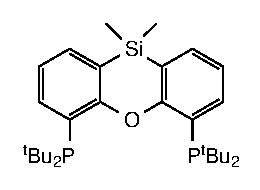
\includegraphics{../Structures/SitBuligand.eps}
%\end{center}
%\end{structure}

This compound was prepared similarly to \tButhixantphos{} using 10,10-dimethyl\-phenoxasilin (0.40 g, 1.8 mmol) giving the title compound as white crystals (0.127 g, 14\%).

\Phosphorusintro{CD2Cl2}
8.4 (s, \XJXX{4}{PSi} = 4.8 Hz).
%\NMRPsinglet{8.42} \fixme{it has silicon satellites? should I add them?}.
\Protonintro{500}{CD2Cl2}
\NMRcoupled{7.87}{d}{7.4}{\SitBucH},
\NMRcoupled{7.53}{d}{7.1}{\SitBuaH},
\NMRcoupled{7.12}{t}{7.5}{\SitBubH},
\NMRPH{1.29}{vt}{5.6}{\SitBuiH},
\NMRsinglet{0.46}{\SitBugH},
\Carbonintro{125}{CD2Cl2}
\NMRPC{164.3}{vt}{11.3}{\SitBueC},
\NMRsinglet{138.5}{\SitBucC},
\NMRsinglet{134.8}{\SitBuaC},
\NMRsinglet{128.0}{\SitBudC},
\NMRsinglet{121.4}{\SitBubC},
\NMRsinglet{119.4}{\SitBufC},
\NMRPC{33.2}{dd}{16.3, 13.9}{\SitBuhC},
\NMRPC{31.0}{vt}{9.6}{\SitBuiC},
\NMRsinglet{-0.09}{\SitBugC}.
HRMS calcd for \ce{C30H49OP2Si} [M + H]$^+$ \emph{m/z} = 515.3022; found = 515.3021.

%%%%%
%C-tBu%
%%%%%

\subsection*{9,9-Dimethyl-4,6-bis(diphenylphosphino)xanthene \\(\tBuxantphos)}

%\begin{structure}[h]
%\begin{center}
%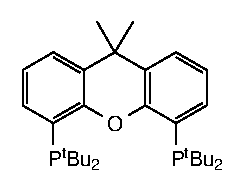
\includegraphics{../Structures/CtBuligand.eps}
%\end{center}
%\end{structure}

9,9-dimethylxanthene (0.50 g, 2.38 mmol) and \gls{TMEDA} (1.07 mL, 7.13 mmol) were dissolved in diethyl ether (20 mL).  Added s-BuLi dropwise causing the reaction to change to yellow then a deep red.  After stirring for 24 hours chlorodi(\emph{tert}-butyl)phosphine (1.36 mL, 7.13 mmol) was added dropwise.  After six days of stirring a white precipitate had formed and a pale yellow solution remained.  The solvent was removed \emph{in vacuo} and the resulting yellow oil was taken up in dichloromethane (20 mL) and washed with degassed water (10 mL).  The aqueous layer was further extracted with dichloromethane (20 mL) and the combined organic layers were washed with water (3 x 10 mL).  The organic layers were dried over magnesium sulfate and the solvent was removed \emph{in vacuo}.  The resulting pale yellow solid was recrystallised from n-propanol yielding the title compound as fine white needles (0.44 g, 37\%).

The \proton{} and \carbon{} NMR data are consistent with the literature values.\cite{Mispelaere2005}  However, the literature reported \phosphorus{} chemical shift is 12.4 ppm.  Due to this discrepancy full characterisation data for this compound is given below.

\Phosphorusintro{CDCl3}
\NMRPsinglet{10.2},
\Protonintro{500}{CDCl3}
\NMRcoupled{7.60}{d}{7.6}{\CtBucH},
\NMRdd{7.38}{7.8}{1.5}{\CtBuaH},
\NMRcoupled{7.03}{t}{7.6}{\CtBubH},
\NMRsinglet{1.57}{\CtBuhH},
\NMRmultiplet{1.21-1.25}{\CtBujH}.
\Carbonintro{125}{CDCl3}
\NMRPC{155.8}{vt}{12.0}{\CtBueC},
\NMRbsinglet{133.7}{\CtBucC},
\NMRPC{130.7}{vt}{2.0}{\CtBufC},
\NMRPC{126.6}{dd}{21.6, 15.4}{\CtBudC},
\NMRsinglet{125.5}{\CtBuaC},
\NMRsinglet{121.5}{\CtBubC},
\NMRbsinglet{35.0}{\CtBugC},
\NMRPC{32.7}{dd}{16.1, 12.7}{\CtBuiC},
\NMRsinglet{31.1}{\CtBuhC},
\NMRPC{30.8}{vt}{18.8}{\CtBujC}.
HRMS calcd for \ce{C31H49OP2} [M+H]$^+$ \emph{m/z} = 499.3253; found = 499.3241.

%%%%%%%%
%Trans ligand%
%%%%%%%%

\subsection*{2,6-bis(di-\emph{tert}-butylphosphino)phenoxathiin}

\begin{structure}[h]
\begin{center}
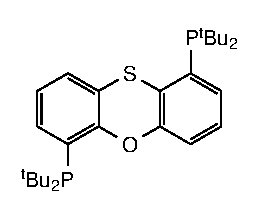
\includegraphics{../Structures/Transthixantphos.eps}
\end{center}
\end{structure}

Phenoxathiin (0.20 g, 1.00 mmol) and TMEDA (0.43 mL, 2.27 mmol) were dissolved in heptane (6 mL).  A solution of \emph{sec}-butyllithium (1.0 M in cyclohexane, 2.27 mL) was added dropwise.  The mixture was stirred for 24 hours resulting in a yellow solution with a white precipitate.  \ce{P^{t}Bu2Cl} (0.55 mL, 2.90 mmol) was added dropwise to the reaction and the resulting mixture was heated at 60 \degC{}  for 24 hours.  The solvent was removed under reduced pressure and the resulting yellow oil was taken up in dichloromethane (10 mL) and washed with degassed water (2 x 10 mL).  The organic layer was dried by passing through a plug of \ce{MgSO4} before removed the solvent \emph{in vacuo}.  The resulting oil was recrystallised from hot n-propanol yielding the title compound as a yellow microcrystalline solid (0.316 g, 65\%).  

\Phosphorusintro{CDCl3}
\NMRcoupled{17.7}{d}{2.2}{\emph{P}CCO}
\NMRcoupled{11.7}{d}{2.3}{\emph{P}CCS}
\Protonintro{500}{CDCl3}
7.49 (d, \J = 7.6 Hz, 1H, Ar),
7.40 (d, \J = 7.3 Hz, 1H, Ar),
7.17 (dd, \J = 7.7 Hz, 1.3 Hz, 1H, Ar),
7.13 (d, \J = 7.6 Hz, 1H, Ar),
7.07 (t, \J = 7.7 Hz, 1H, Ar),
6.94 (t, \J = 7.6 Hz, 1H, Ar),
1.21 (d, \J = 12.3 Hz, 18H, \StBuiH),
1.20 (d, \J = 12.0 Hz, 18H, \StBuiH).
\Carbonintro{150}{CDCl3}
156.4 (d, \JPC = 17.9 Hz, 1C, Ar),
151.6 (d, \JPC = 10.4 Hz, 1C, Ar),
134.1 (s, 1C, Ar),
134.0 (s, 1C, Ar),
133.8 (s, 1C, Ar),
130.5 (d, \JPC = 3.4 Hz, 1C, Ar),
127.9 (s, 1C, Ar),
126.2 (d, \JPC = 31.8 Hz, 1C, Ar),
125.6 (d, \JPC = 7.0 Hz, 1C, Ar),
122.8 (s, 1C, Ar),
122.3 (d, \JPC = 17.9 Hz, 1C, Ar),
119.4 (s, 1C, Ar)
33.1 (d, \JPC = 21.4 Hz, \StBuhC),
32.4 (d, \JPC = 23.7 Hz, \StBuhC),
30.7 (d, \JPC = 15.1 Hz, \StBuiC),
30.4 (d, \JPC = 14.4 Hz, \StBuiC).

%%%%%%%%
% C-tBu acid %
%%%%%%%%
\subsection*{Synthesis of \texorpdfstring{[(\tBuxantphos)H]\ce{CH(SO2CF3)}} t}

%Protonated 4,6-bis(di-\emph{tert}-butylphosphino)-9,9-dimethylxanthene\\(\emph{t}-Bu-xantphos) with \ce{CH2(SO2CF3)2}}

%\begin{structure}[h]
%\begin{center}
%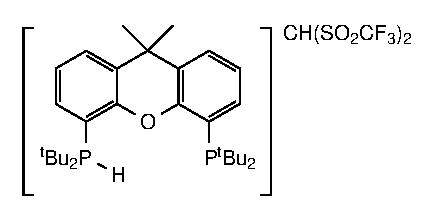
\includegraphics{../Structures/CtBuH.eps}
%\end{center}
%\end{structure}

A solution of \ce{CH2(SO2CF3)2} (0.009 g, 0.032 mmol) in \ce{CDCl3} (0.5 mL) was added to \tBuxantphos{} (0.016 g, 0.032 mmol)  in an NMR tube.  The reaction was instantaneous and quantitative conversion was observed by NMR spectroscopy.  Removal of the solvent \emph{in vacuo} gave the product as a white solid in quantitative yield.  

%Reaction3013

%Phosphorus
\Phosphorusintro{CDCl3}
17.4 (bs).
%Proton
\Protonintro{600}{CDCl3}
\NMRmultiplet{9.05 - 8.09}{P\emph{H}},
%\NMRPH{8.7}{vt}{470.6}{P\emph{H}}, \fixme{kind of not really}
\NMRmultiplet{7.67-7.74}{4H, Ar},
\NMRbsinglet{7.39}{2H, Ar},
\NMRbsinglet{4.06}{C\emph{H}\ce{(SO2CF3)2}},
\NMRsinglet{1.65}{\CtBuhH},
\NMRmultiplet{1.37-1.43}{\CtBujH}.
%Fluorine
\Fluorineintro{CDCl3}
\NMRsinglet{-80.9}{C\emph{F}\sub{3}}
%Carbon
\Carbonintro{150}{CDCl3}
\NMRmultiplet{153.6-153.8}{\CtBueC},
\NMRbcarbon{132.5},
\NMRbcarbon{130.3},
\NMRbcarbon{125.0},
\NMRCF{121.0}{quartet}{317.9}{CH\ce{(SO2}\emph{C}\ce{F3)2}},
\NMRsinglet{54.1}{\emph{C}H\ce{(SO2CF3)2}},
\NMRsinglet{35.5}{\CtBugC},
\NMRbsinglet{34.0}{\CtBuiC},
\NMRsinglet{30.8}{\CtBuhC},
\NMRbsinglet{29.4}{\CtBujC}.
HRMS calcd for \ce{C31H49OP2} [M]$^+$ \emph{m/z} = 499.3253; found = 499.3254.

%%%%%%%
%S-tBu acid%
%%%%%%%
\subsection*{Synthesis of \texorpdfstring{[(\tButhixantphos)H]\ce{CH(SO2CF3)}} t}

%\begin{structure}[h]
%\begin{center}
%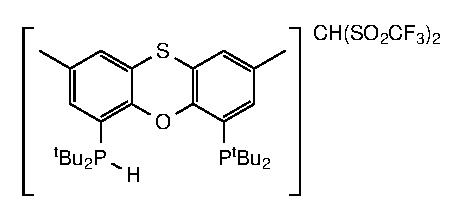
\includegraphics{../Structures/StBuH.eps}
%\end{center}
%\end{structure}

%Reaction 1093
This product was synthesised similarly to [\tBuxantphos(H)]\ce{CH(SO2CF3)2} using \tButhixantphos{} (0.041 g, 0.079 mmol) giving the title compound in quantitative yield as a pale yield solid.  X-ray quality crystals were grown by performing the reaction in \ce{C6D6} and allowing the solvent to slowly evaporate.  

\Phosphorusintro{CD2Cl2}
\NMRPsinglet{15.8}
\Protonintro{500}{CD2Cl2}
\NMRmultiplet{8.99}{P\emph{H}},
\NMRsinglet{7.29}{\StBuaH},
\NMRsinglet{7.22}{\StBucH},
\NMRsinglet{3.83}{\ce{C\emph{H}(SO2CF3)}},
\NMRsinglet{2.36}{\StBugH},
\NMRmultiplet{1.41-1.44}{\StBuiH}.
\Carbonintro{125}{CD2Cl2}
\NMRsinglet{152.9}{\StBueC},
\NMRsinglet{136.2}{\StBubC},
\NMRsinglet{132.5}{\StBuaC},
\NMRsinglet{131.8}{\StBucC},
\NMRsinglet{122.2}{\StBufC},
\NMRCF{121.5}{quartet}{325.6}{\ce{CF3}},
\NMRsinglet{115.3}{\StBudC},
\NMRsinglet{34.4}{\StBuhC},
\NMRsinglet{29.5}{\StBuiC}.
One peak (\emph{C}\ce{H(SO2CF3)}) obscured by solvent.
HRMS calcd for \ce{C30H47OP2S} [M]$^+$ \emph{m/z} = 517.2817; found = 517.2817.

%%%%%%%%
% Si-tBu acid %
%%%%%%%%
\subsection*{Synthesis of \texorpdfstring{[(\tBusixantphos)H]\ce{CH(SO2CF3)}} t}

%\begin{structure}[h]
%\begin{center}
%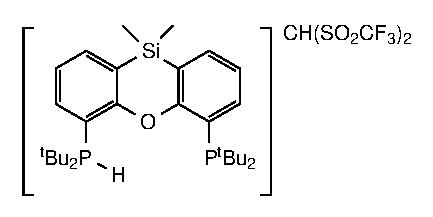
\includegraphics{../Structures/SitBuH.eps}
%\end{center}
%\end{structure}

%Reaction4010\\
[\tBuSixantphos(H)]\ce{CH(SO2CF3)2} was synthesised in a similar manner to [\tBuxantphos(H)]\ce{CH(SO2CF3)} using \tBusixantphos{} (0.020 g, 0.039 mmol).  The product was produced as a white solid in quantitative yield.  

%Phosphorus
\Phosphorusintro{CDCl3}
\NMRPsinglet{14.3}
%Proton
\Protonintro{500}{CDCl3}
\NMRmultiplet{9.57}{P\emph{H}},
\NMRmultiplet{7.85-7.87}{\SitBucH},
\NMRHH{7.79}{d}{6.6}{\SitBuaH},
\NMRHH{7.41}{t}{7.5}{\SitBubH},
\NMRbsinglet{4.06}{C\emph{H}\ce{(SO2CF3)2}},
\NMRPH{1.43}{vt}{7.5}{\SitBuiH},
\NMRsinglet{0.53}{\SitBugH}.
%Fluorine
\Fluorineintro{CDCl3}
\NMRsinglet{-80.8}{C\emph{F}\sub{3}}
%Carbon
\Carbonintro{125}{CDCl3}
\NMRPC{161.5}{vt}{5.3}{\SitBueC},
\NMRsinglet{139.1}{\SitBuaC},
\NMRsinglet{136.9}{\SitBucC},
\NMRPC{124.0}{vt}{2.4}{\SitBubC},
\NMRsinglet{121.1}{\SitBufC},
\NMRCF{121.1}{quartet}{327.2}{CH\ce{(SO2}\emph{C}\ce{F3)2}},
\NMRbsinglet{115.0}{\SitBudC},
\NMRsinglet{53.6}{\emph{C}H\ce{(SO2CF3)2}},
\NMRPC{34.2}{vt}{3.9}{\SitBuhC},
\NMRPC{29.5}{vt}{4.3}{\SitBuiC},
\NMRsinglet{-0.4}{\SitBugC}.
HRMS calcd for \ce{C30H49OP2Si} [M]$^+$ \emph{m/z} = 515.3022; found = 515.3023.

%%%%%%
%SitBu Se%
%%%%%%

%Reaction6008
\subsection*{\tBuSixantphos Se}
%\fixme{Correct this name}

%\begin{structure}[h]
%\begin{center}
%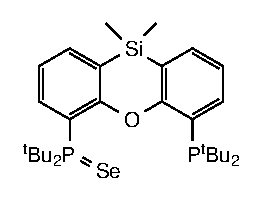
\includegraphics{../Structures/SitBuSe.eps}
%\end{center}
%\end{structure}

A solution of \tBuxantphos{} (0.031 g, 0.060 mmol) in toluene (5 mL) was added to grey selenium (0.095 g, 1.20 mmol) in toluene (5 mL).  The reaction was heated to reflux with stirring for 3 days.  The resulting yellow solution was allowed to cool, filtered and reduced \emph{in vacuo} to give a pale yellow solid (0.036 g, 100\%).

\phosphorus{} NMR (121 MHz, 1:1, \ce{CDCl3}:\ce{CD2Cl2}): $\delta$
%\Phosphorusintro{1:1, CDCl3:CD2Cl2}
\NMRPasysinglet{15.9}{P},
102.7 (s, \JPSe{} = 689.1 Hz, \ce{P=Se}).
\proton{} NMR (300 MHz, 1:1, \ce{CDCl3}:\ce{CD2Cl2}): $\delta$
%\Protonintro{300}{1:1 CDCl3:CD2Cl2}
\NMRbsinglet{9.13}{1H, Ar},
7.81 (d, \J{} = 7.5 Hz, 1H, Ar),
%\NMRcoupled{7.81}{d}{7.5}{1H, Ar},
\NMRmultiplet{7.66-7.16}{4H, Ar},
\NMRcoupled{1.61}{d}{22.5}{\ce{P(=Se)C(C\emph{H3})3}},
\NMRcoupled{1.10}{d}{11.5}{\SitBuiH},
\NMRsinglet{0.36}{\SitBugH},
\NMRsinglet{0.07}{\SitBugH}.
HRMS calcd for \ce{C30H49OP2SeSi} [M+H]$^+$ \emph{m/z} = 595.2190; found = 595.2172.

%%%%%%
%StBu Se%
%%%%%%

%Reaction4026, 6009
\subsection*{\tBuThixantphos{}Se}
%\fixme{Correct this name}
%\begin{structure}[h]
%\begin{center}
%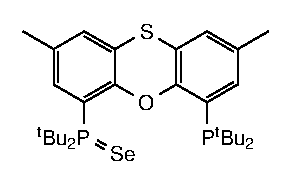
\includegraphics{../Structures/StBuSe.eps}
%\end{center}
%\end{structure}

A solution of \tButhixantphos{} (0.042 g, 0.081 mmol) in toluene (5 mL) was added to grey selenium (0.128 g, 1.62 mmol) in toluene (5 mL).  The reaction was heated to reflux with stirring for 3 days.  The resulting yellow solution was allowed to cool, filtered and reduced \emph{in vacuo} to give the title compound as a yellow solid (0.047 g, 98\%).   

\Phosphorusintro{CDCl3}
\NMRPasysinglet{11.7}{P},
101.9 (s, \JPSe{} = 698.5 Hz, \ce{P=Se}).
\Protonintro{300}{CDCl3}
\NMRcoupled{8.85}{d}{16.2}{\ce{P(=Se)}CC\emph{H}},
\NMRsinglet{7.26}{1H, Ar},
\NMRsinglet{6.96}{1H, Ar},
\NMRsinglet{6.89}{1H, Ar},
\NMRsinglet{2.27}{3H, \StBugH},
\NMRsinglet{2.25}{3H, \StBugH},
\NMRcoupled{1.62}{d}{16.6}{18H, \ce{P(=Se)C(C\emph{H3})3}},
\NMRcoupled{1.15}{d}{11.9}{18H, \StBuiH}.
HRMS calcd for \ce{C31H49OP2SSe} [M+H]$^+$ \emph{m/z} = 597.1984; found = 597.1919.

%%%%%%
%CtBu Se%
%%%%%%

%Reaction4031, 6010
\subsection*{\tBuXantphos{}Se}

%\fixme{Correct this name}
%\begin{structure}[h]
%\begin{center}
%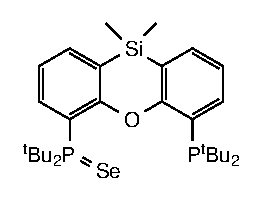
\includegraphics{../Structures/CtBuSe.eps}
%\end{center}
%\end{structure}

A solution of \tBuxantphos{} (0.041 g, 0.082 mmol) in toluene (5 mL) was added to grey selenium (0.130 g, 1.65 mmol) in toluene (5 mL).  The reaction was heated to reflux with stirring for 3 days.  The resulting yellow solution was allowed to cool, filtered and reduced \emph{in vacuo} to give a pale yellow solid (0.038 g, 80\%).    

\begin{sloppypar}
\phosphorus{} NMR (121 MHz, 1:1, \ce{CDCl3}:\ce{CD2Cl2}): $\delta$
\NMRPasysinglet{10.6}{P},
101.9 (s, \JPSe{} = 697.1 Hz, \ce{P=Se}).
%\NMRPasysinglet{101.9}{\ce{P=Se}}.
\proton{} NMR (500 MHz, 1:1, \ce{CDCl3}:\ce{CD2Cl2}): $\delta$
\NMRdd{9.26}{17.4}{7.8}{P(=Se)CC\emph{H}},
\NMRcoupled{7.67}{d}{7.6}{\CtBucH},
\NMRcoupled{7.60}{d}{7.5}{P(=Se)CCCC\emph{H}},
\NMRcoupled{7.50}{d}{7.5}{PCCCC\emph{H}},
\NMRcoupled{7.24}{t}{7.8}{P(=Se)CCC\emph{H}},
\NMRcoupled{7.19}{t}{7.6}{\CtBubH},
\NMRcoupled{1.66}{d}{16.6}{\ce{P(=Se)C(C\emph{H3})3}},
\NMRsinglet{1.57}{\CtBuhH},
\NMRcoupled{1.19}{d}{11.8}{\CtBujH}.
\carbon{} NMR (125 MHz, 1:1 \ce{CDCl3}:\ce{CD2Cl2}): $\delta$
%\Carbonintro{125}{1:1, CDCl3:CD2Cl2},
\NMRPC{157.0}{d}{21.1}{\CtBueC},
\NMRsinglet{154.2}{P(=Se)C\emph{C}O},
\NMRPC{143.5}{d}{11.6}{P(=Se)C\emph{C}H},
\NMRsinglet{136.0}{\CtBucC},
\NMRsinglet{132.8}{PCC\emph{C}C(bridge)},
\NMRPC{132.0}{d}{4.8}{P(=Se)CC\emph{C}C(bridge)},
\NMRPC{129.2}{d}{2.4}{P(=Se)CCC\emph{C}H},
\NMRsinglet{126.3}{PCCC\emph{C}H},
\NMRPC{125.3}{d}{35}{\CtBudC},
\NMRsinglet{123.2}{2C, P(=Se)CC\emph{C}H, PCC\emph{C}H},
\NMRPC{115.4}{d}{39.8}{P(=Se)\emph{C}(Ar)},
\NMRPC{39.2}{d}{34.6}{P(=Se)\emph{C}(CH3)3},
\NMRsinglet{35.3}{\emph{C}(bridge)},
\NMRPC{33.5}{d}{26.9}{\CtBuiC},
\NMRPC{31.2}{d}{15.4}{\CtBujC},
\NMRdd{30.9}{7.7}{2.0}{P(=Se)C(\emph{C}\ce{H3)3}}.
\NMRsinglet{30.8}{C(bridge)\emph{C}\ce{H3}}.
HRMS calcd for \ce{C31H49OP2Se} [M+H]$^+$ \emph{m/z} = 579.2421; found = 579.2381.
\end{sloppypar}

\section{Silver Complexes}
\label{section:experimental:silver}

%%%%%%
%AgCl StBu%
%%%%%%

%Reaction3002
%\newpage{}

\subsection*{[Ag(\tButhixantphos)Cl]}

%3003
%\begin{structure}[h]
%\begin{center}
%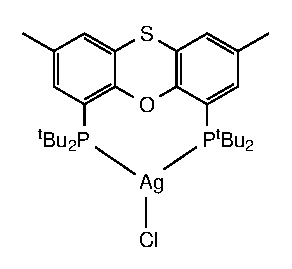
\includegraphics{../Structures/StBuSilverChloride.eps}
%\end{center}
%\end{structure}

This reaction was carried out in the dark.  \tBuThixantphos{} (88 mg, 0.17 mmol) and silver chloride (24 mg, 0.17 mmol) were combined \ce{CH2Cl2} (4 mL) in a Schlenk tube.  After 5 days stirring the solution was passed through a plug of alumina, washing with dichloromethane (4 x 1 mL).  The solvent was removed \emph{in vacuo} giving a cloudy oil.  The oil was triturated with hexane (2 mL) yielding the title compound as a white powder (94 mg, 84\%).  The resulting silver complex is light sensitive and care should be taken to exclude light.

\begin{sloppypar}
%Phosphorus
\Phosphorusintro{CDCl3}
\NMRAgP{21.81}{406.7}{469.6}.
%Proton
\Protonintro{600}{CDCl3}
\NMRPH{7.39}{d}{1.0}{\StBucH},
\NMRPH{7.11}{d}{1.6}{\StBuaH},
\NMRsinglet{2.31}{\StBugH}
\NMRmultiplet{1.41}{\StBuiH}.
%Carbon
\Carbonintro{150}{CDCl3}
\NMRPC{155.5}{vt}{6.6}{\StBueC},
\NMRPC{134.8}{d}{4.9}{\StBucC},
\NMRPC{133.1}{d}{1.5}{\StBubC},
\NMRsinglet{130.3}{\StBuaC},
\NMRPC{122.8}{vt}{3.0}{\StBufC},
\NMRmultiplet{120.9}{\StBudC}
\NMRmultiplet{35.3}{\StBuhC}
\NMRPC{30.9}{vt}{5.6}{\StBuiC},
\NMRsinglet{20.8}{\StBugC}.
HRMS calcd for \ce{C30H46OP2SAg} [M-Cl]$^+$ \emph{m/z} = 623.1796; found = 623.1805.
\end{sloppypar}

%%%%%%%%
% AgCl SitBu %
%%%%%%%%

%Reaction3003
%\newpage{}
%\subsection*{[Ag(\tBusixantphos)Cl]}
%\begin{structure}[h]
%\begin{center}
%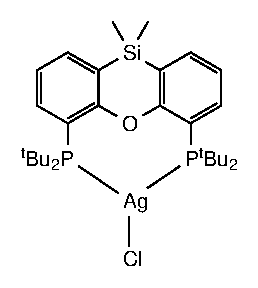
\includegraphics{../Structures/SitBuSilverChloride.eps}
%\end{center}
%\end{structure}

\subsection*{[Ag(\tBusixantphos)Cl]}

This reaction was carried out in the dark.  \tBuSixantphos{} and silver chloride were combined in an NMR tube, dissolved in \ce{CDCl3}, and sonicated for 5 mins.  After four days the reaction was sonicated for 6 x 5 mins.  The solution was decanted and the resulting solid was washed with dichloromethane (3 x 1 mL).  The solvent was removed \emph{in vacuo} yielding the title compound as a white solid (31 mg, 97\%).  The resulting silver complex is light sensitive and care should be taken to exclude light.

\begin{sloppypar}
%Phosphorus
\Phosphorusintro{CDCl3}
\NMRAgP{24.2}{408.1}{471.1}
%Proton
\Protonintro{600}{CDCl3}
\NMRmultiplet{7.88}{\SitBucH},
\NMRdd{7.61}{7.0}{1.8}{\SitBuaH},
\NMRHH{7.21}{t}{7.3}{\SitBubH},
\NMRmultiplet{1.42}{\SitBuiH},
\NMRsinglet{0.46}{\SitBugH}.
%Carbon
\Carbonintro{150}{CDCl3}
\NMRPC{163.9}{vt}{5.2}{\SitBueC},
\NMRPC{138.2}{d}{4.4}{\SitBucC},
\NMRsinglet{136.3}{\SitBuaC},
\NMRsinglet{122.2}{\SitBufC},
\NMRsinglet{122.1}{\SitBubC},
\NMRmultiplet{120.5}{\StBudC}
\NMRmultiplet{35.5}{\StBuhC}
\NMRPC{31.0}{vt}{5.6}{\StBuiC},
\NMRsinglet{-1.3}{\StBugC}.
HRMS calcd for \ce{C30H48OP2Ag} [M-Cl]$^+$ \emph{m/z} = 621.2001; found = 621.2021.
\end{sloppypar}

%%%%%%%
%AgCl CtBu%
%%%%%%%

%Reaction3017
%\newpage{}
\subsection*{[Ag(\tBuxantphos)Cl]}

%\begin{structure}[h]
%\begin{center}
%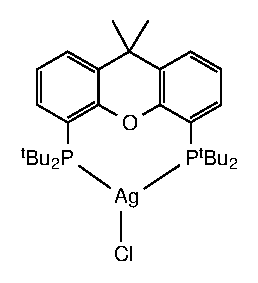
\includegraphics{../Structures/CtBuSilverChloride.eps}
%\end{center}
%\end{structure}

This reaction was carried out in the dark.  \tBuXantphos{} (0.017 g, 0.034 mmol) and silver chloride (0.005 g, 0.035 mmol) were combined in an NMR tube and dissolved in \ce{CDCl3}.  After 48 hours the reaction mixture was sonicated 10 x 5 mins.  The solution was decanted and the resulting solid was dried under reduced pressure leaving the title compound as a white powder (0.017 g, 78\%).  The resulting silver complex is light sensitive and care should be taken to exclude light.

%Phosphorus
\Phosphorusintro{CDCl3}
\NMRAgP{20.7}{409.3}{472.2}
%Proton
\Protonintro{500}{CDCl3}
\NMRPH{7.68}{d}{6.9}{\CtBucH},
\NMRdd{7.53}{7.6}{1.2}{\CtBuaH},
\NMRHH{7.19}{t}{7.7}{\CtBubH},
\NMRsinglet{1.56}{\CtBuhH},
\NMRmultiplet{1.40-1.43}{\CtBujH}.
%Carbon
\Carbonintro{125}{CDCl3}
\NMRPC{156.5}{vt}{6.5}{\CtBueC},
\NMRmultiplet{133.7}{\CtBucC},
\NMRsinglet{130.7}{\CtBufC},
\NMRsinglet{126.8}{\CtBuaC},
\NMRsinglet{122.7}{\CtBubC},
\NMRmultiplet{119.3}{\CtBudC},
\NMRmultiplet{35.6}{\CtBugC},
\NMRmultiplet{35.1}{\CtBuiC},
\NMRPC{30.8}{vt}{5.6}{\CtBujC},
\NMRsinglet{28.5}{\CtBuhC}.
HRMS calcd for \ce{C31H48OP2Ag} [M-Cl]$^+$ \emph{m/z} = 605.2226; found = 605.2163.

%%%%%%%%%
% AgBF4 SitBu %
%%%%%%%%%

%Reaction3009
\subsection*{\texorpdfstring{[Ag(\tBusixantphos)]\ce{BF4}} A}

%\begin{structure}[h]
%\begin{center}
%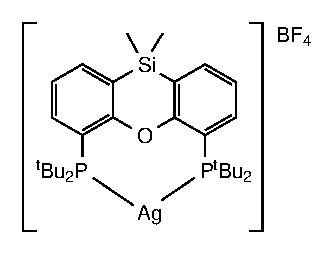
\includegraphics{../Structures/SitBuSilverBF4.eps}
%\end{center}
%\end{structure}

This reaction was carried out in the dark.  \tBuSixantphos{} (0.027 g, 0.052 mmol) and silver tetrafluoroborate (0.010, 0.052 mmol) were combined in an NMR tube and dissolved in \ce{CDCl3}.  After 3 days the reaction was complete by NMR spectroscopy.  The solution was removed under reduced pressure yielding the title compound as a white solid (0.024 g, 0.034 mmol, 64\%).

%Phosphorus
\Phosphorusintro{CDCl3}
\NMRAgP{31.5}{482.9}{557.4}.
%Proton
\Protonintro{500}{CDCl3}
\NMRbsinglet{7.84}{\SitBucH},
\NMRHH{7.73}{d}{6.8}{\SitBuaH},
\NMRHH{7.34}{t}{7.3}{\SitBubH},
\NMRPH{1.40}{vt}{15.9}{\SitBuiH},
\NMRsinglet{0.49}{\SitBugH}.
%Carbon
\Carbonintro{125}{CDCl3}
\NMRPC{162.3}{vt}{8.7}{\SitBueC},
\NMRsinglet{138.2}{\SitBuaC},
\NMRPC{138.1}{d}{6.7}{\SitBucC},
\NMRPC{123.1}{d}{1.9}{\SitBubC},
\NMRsinglet{122.1}{\SitBufC},
\NMRmultiplet{118.4}{\SitBudC},
\NMRmultiplet{35.7}{\SitBuhC}, %Virtual triplet of doublet?
\NMRmultiplet{30.9}{\SitBuiC},
\NMRsinglet{-0.6}{\SitBugC}.
%Fluorine
\Fluorineintro{CDCl3}
\NMRsinglet{-151.9}{\ce{BF4-}}.
HRMS calcd for \ce{C30H48OP2AgSi} [M-\ce{BF4-}]$^+$ \emph{m/z} = 621.2001; found = 621.2032.

%%%%%%%%
%AgBF4 StBu%
%%%%%%%%

%Reaction3008
%\newpage{}

\subsection*{\texorpdfstring{[Ag(\tButhixantphos)]\ce{BF4}} A}

%\begin{structure}[h]
%\begin{center}
%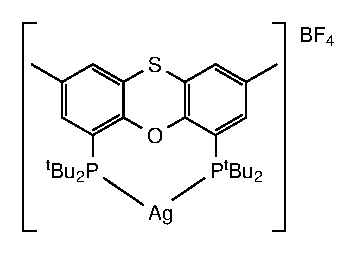
\includegraphics{../Structures/StBuSilverBF4.eps}
%\end{center}
%\end{structure}

This reaction was carried out in the dark.  A solution of \tButhixantphos{} (0.026 g, 0.050 mmol) in 0.5 mL of \ce{CDCl3} was added to silver tetrafluoroborate (0.010 g, 0.051 mmol) in an NMR tube.  After 3 days the reaction NMR showed complete conversion into the title complex.  The solvent was removed under reduced pressure yielding the product as a white solid (0.030 g, 0.042 mmol, 84\%).

\begin{sloppypar}
%Phosphorus
\Phosphorusintro{CDCl3}
\NMRAgP{28.4}{486.7}{562.2}.
%Proton
\Protonintro{500}{CDCl3}
\NMRsinglet{7.32}{\StBucH},
\NMRsinglet{7.16}{\StBuaH},
\NMRsinglet{2.33}{\StBugH},
\NMRPH{1.40}{vt}{15.8}{\StBuiH}.
%Carbon
\Carbonintro{125}{CDCl3}
\NMRPC{153.9}{vt}{11.0}{\StBueC},
\NMRPC{134.4}{d}{1.7}{\StBubC},
\NMRPC{134.2}{d}{6.30}{\StBucC},
\NMRsinglet{131.1}{\StBuaC},
\NMRsinglet{122.3}{\StBufC},
\NMRmultiplet{119.4}{\StBudC}, %virtual triplet of doublets?
\NMRmultiplet{35.5}{\StBuhC},
\NMRmultiplet{30.8}{\StBuiC},
\NMRsinglet{20.7}{\StBugC}.
%Fluorine
\Fluorineintro{CDCl3}
\NMRsinglet{151.3}{\ce{BF4-}}.
HRMS calcd for \ce{C30H46OP2SAg} [M-\ce{BF4-}]$^+$ \emph{m/z} = 623.1796; found = 623.1826.
\end{sloppypar}

%%%%%%%%
%AgBF4 CtBu%
%%%%%%%%

%Reaction3016
%\newpage{}
\subsection*{\texorpdfstring{[Ag(\tBuxantphos)]\ce{BF4}} A} %\fixme{check name}

%\begin{structure}[h]
%\begin{center}
%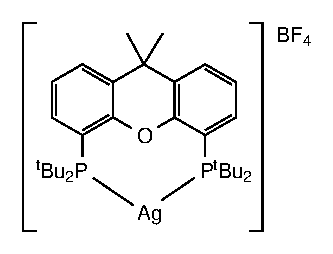
\includegraphics{../Structures/CtBuSilverBF4.eps}
%\end{center}
%\end{structure}

This reaction was carried out in the dark as silver compounds are typically light sensitive.  \tBuXantphos{} (0.017 g, 0.034 mmol) and silver tetrafluoroborate (0.008 g, 0.041 mmol) were combined in an NMR tube and dissolved in \ce{CDCl3}.  After 48 hours the reaction was complete by NMR spectroscopy.  The solvent was removed under reduced pressed yielding a white solid in quantitative yield.  

%Phosphorus
\Phosphorusintro{CDCl3}
\NMRAgP{27.6}{486.3}{561.1}
%Proton
\Protonintro{500}{CDCl3}
\NMRmultiplet{7.63-7.67}{\CtBuaH, \CtBucH},
\NMRHH{7.29}{t}{7.7}{\CtBubH},
\NMRsinglet{1.59}{\CtBuhH},
\NMRmultiplet{1.39-1.42}{\CtBujH}.
%Carbon
\Carbonintro{125}{CDCl3}
\NMRPC{154.9}{vt}{5.6}{\CtBueC},
\NMRPC{133.5}{vt}{1.9}{\CtBucC},
\NMRPC{133.5}{d}{5.8}{\CtBufC},
\NMRsinglet{128.4}{\CtBuaC},
\NMRsinglet{123.8}{\CtBubC},
\NMRsinglet{117.8}{\CtBudC},
\NMRPC{35.6}{vtd}{5.3, 2.4}{\CtBugC},
\NMRmultiplet{35.3}{\CtBuiC},
\NMRmultiplet{30.6}{\CtBujC},
\NMRsinglet{29.4}{\CtBuhC}.
%Fluorine
\Fluorineintro{CDCl3}
\NMRsinglet{-151.9}{\ce{BF4-}}
HRMS calcd for \ce{C31H48OP2Ag} [M-\ce{BF4-}]$^+$ \emph{m/z} = 605.2226; found = 605.2217.

\subsection*{Reaction of \texorpdfstring{[Ag(\tBusixantphos)]\ce{BF4}} A with LiCCPh}

A solution of n-butyllithium in cyclohexanes (1.6 M 0.12 mL) was added to a solution of phenylacetylene (0.021 mL) in THF (40 mL).  The mixture was stirred for 10 minutes, then a solution of [Ag(\tBusixantphos)]\ce{BF4} (0.34 g) in THF (2.0 mL) was added.  The reaction mixture was stirred in the dark for 2 hours.  The solvent was removed \emph{in vacuo} and the residue taken up in acetone-\ce{d6} for NMR analysis.   

\begin{sloppypar}
\Phosphorusintro{acetone-d6}
\NMRAgP{26.4}{418.5}{482.9}
\Protonintro{500}{acetone-d6}
\NMRmultiplet{8.06}{2H, Ar},
\NMRcoupled{7.86}{dd}{7.1, 1.5}{2H, Ar},
\NMRcoupled{7.41}{t}{7.4}{\SitBubH},
\NMRmultiplet{1.47-1.45}{\SitBuiH},
\NMRsinglet{0.51}{\SitBugH}.
\Fluorineintro{acetone-d6}
\NMRsinglet{-152.3}{\ce{BF4-}}.
\end{sloppypar}

\subsection*{Reaction of \texorpdfstring{[Ag(\tButhixantphos)]\ce{BF4}} A with LiCCPh}

A solution of n-butyllithium in cyclohexanes (1.6 M 0.11 mL) was added to a solution of phenylacetylene (0.020 mL) in THF (40 mL).  The mixture was stirred for 10 minutes, then 17 mL of the solution was added to a solution of [Ag(\tButhixantphos)]\ce{BF4} in (0.055 g) in THF (3.0 mL).  The reaction mixture was stirred in the dark for 12 hours.  The solvent was removed \emph{in vacuo} and the residue taken up in acetone-\ce{d6} or \ce{C6D6} for NMR analysis.   

\begin{sloppypar}
\Phosphorusintro{C6D6}
23.4, (bs)
19.9, (bs)
\Protonintro{300}{C6D6}
\NMRmultiplet{7.7-6.8}{6H, Ar},
\NMRbsinglet{1.96}{\StBugH},
\NMRbsinglet{1.42}{\StBuiH}.
\Fluorineintro{C6D6}
\NMRsinglet{-156.9}{\ce{BF4-}}
\end{sloppypar}

\begin{sloppypar}
\Phosphorusintro{acetone-d6}
\NMRAgP{23.1}{410.3}{474.1}.
\Protonintro{300}{acetone-d6}
\NMRsinglet{7.61}{2H, Ar}
\NMRsinglet{7.36}{2H, Ar}
\NMRsinglet{2.39}{\StBugH},
\NMRmultiplet{1.51-1.46}{\StBuiH}.
\Fluorineintro{acetone-d6}
\NMRsinglet{-152.1}{\ce{BF4-}}.
\end{sloppypar}

\subsection*{Reaction of \texorpdfstring{[Ag(\tBuxantphos)]\ce{BF4}} A with LiCCPh}

A solution of n-butyllithium in cyclohexanes (1.6 M 0.11 mL) was added to a solution of phenylacetylene (0.020 mL) in THF (40 mL).  The mixture was stirred for 10 minutes, then 16.2 mL of the solution was added to a solution of [Ag(\tBuxantphos)]\ce{BF4} in (0.051 g) in THF (3.0 mL).  The reaction mixture was stirred in the dark for 12 hours.  The solvent was removed \emph{in vacuo} and the residue taken up in acetone-\ce{d6} for NMR analysis.   

\begin{sloppypar}
\Phosphorusintro{acetone-d6}
\NMRAgP{20.7}{407.4}{471.1}.
\Protonintro{500}{acetone-d6}
\NMRcoupled{7.86}{d}{7.5}{2H, Ar},
\NMRcoupled{7.76}{dd}{7.6, 0.9}{2H, Ar},
\NMRcoupled{7.37}{t}{7.6}{\CtBubH},
\NMRsinglet{1.61}{\CtBuhH},
\NMRmultiplet{1.46-1.44}{\CtBujH}.
\Fluorineintro{acetone-d6}
\NMRsinglet{-152.6}{\ce{BF4-}}.
\end{sloppypar}

%\fixme{Need to check and get all of the couplings}
%\fixme{Make sure that all of the proton couplings around all of the rings have consistent PH or HH}
%\fixme{Consider using numbering}
%\fixme{check how on earth to write up all of the tBu couplings...}

%%%%%%%%
%PdCl2 StBu %
%%%%%%%%
%\newpage{}
%\subsection*{\emph{t}-Bu-thixantphospalladiumdichloride, 2020} \fixme{check name}
%\begin{structure}[h]
%\begin{center}
%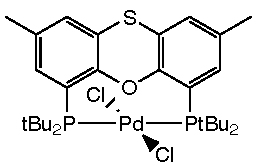
\includegraphics{../Structures/PdCl2(s(tBu)2)_complex.pdf}
%\end{center}
%\end{structure}

%\fixme{StBu ligand} (36 mg, 0.070 mmol) and \ce{[Pd(COD)Cl2]} (20 mg, 0.070 mmol) were combined in an NMR tube and dissolved in \ce{C6D6} and heated to 60\degC{} for 48 hours.  The solvent was removed in vacuo yielding the title compound as a dark red solid (37 mg, 77\%).

%Phosphorus
%\Phosphorusintro{C6D6}
%\NMRPsinglet{41.9}
%Proton
%\Protonintro{500}{C6D6}
%\NMRsinglet{7.17}{PC(Ar)\emph{H}},
%\NMRsinglet{7.15}{SCC\emph{H}}
%\NMRsinglet{2.33}{C(Ar)\ce{C\emph{H}3}}
%\NMRPH{1.59}{vt}{7.1}{PCC\emph{H}\sub{3}}
%Carbon
%\Carbonintro{125}{CDCl3}
%\NMRPC{155.1}{vt}{4.8}{\emph{C}O}
%\NMRsinglet{134.4}{PC(Ar)\emph{C}H}
%\NMRPC{133.4}{vt}{\fixme{?}}{\emph{C}(Ar)\ce{CH3}}
%\NMRsinglet{130.4}{SC\emph{C}H})
%\NMRmultiplet{123.5}{P\emph{C}(Ar)}
%\NMRPC{123.1}{vt}{3.0}{\emph{C}S}
%\NMRPC{39.5}{vt}{5.8}{P\emph{C}C\ce{H3}}
%\NMRsinglet{31.2}{PC\emph{C}\ce{H3}}
%\NMRsinglet{20.7}{C(Ar)\emph{C}\ce{H3}}

%\fixme{IR, EA, 1H, 31P, 13C, MS}
%\fixme{Redraw complex with new parameters}
%\fixme{Check solvent}


\section{Rhodium Complexes}

%%%%%%%%
%Rh(SitBu)Cl%
%%%%%%%%

\subsection*{[Rh(\tBusixantphosk)Cl]}

%\begin{structure}[h]
%\begin{center}
%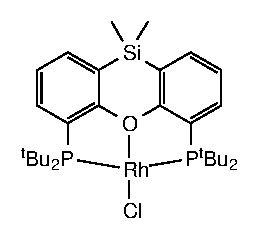
\includegraphics{../Structures/SitBuRhCl.eps}
%\end{center}
%\end{structure}

%7002, 7014%
A solution of \tBusixantphos{} (0.032 g, 0.062 mmol) in \ce{C6D6} was added to solid \ce{[Rh(coe)2Cl]_{n}} (0.027 g, 0.075 mmol, 1.2 eq. of Rh) in a Young's tap NMR tube.  The tube was sealed under argon and heated to 60 \degC{} for 24 hours.  The solution was decanted and the solvent removed \emph{in vacuo} to yield the title compound as a dark red solid in quantitative yield (0.041 g, 0.062 mmol, 100\%).

\Phosphorusintro{C6D6}
\NMRRhP{44.2}{140.0}.
\Protonintro{600}{C6D6}
\NMRmultiplet{8.05}{\SitBucH},
\NMRcoupled{7.13}{dd}{6.8, 1.8}{\SitBuaH},
\NMRcoupled{6.84}{t}{7.2}{\SitBubH},
\NMRPH{1.69}{vt}{13.5}{\SitBuiH},
\NMRsinglet{0.07}{\SitBugH}.
\Carbonintro{125}{C6D6}
\NMRPC{169.5}{\SitBueC},
\NMRsinglet{138.4}{\SitBucC},
\NMRsinglet{136.0}{\SitBuaC},
\NMRmultiplet{127.0}{\SitBudC},
\NMRsinglet{122.8}{\SitBubC},
\NMRPC{121.5}{\SitBufC},
\NMRPC{37.7}{vt}{9.9}{\SitBuhC},
\NMRPC{31.0}{vt}{8.1}{\SitBuiC},
\NMRsinglet{-0.7}{\SitBugC}.
HRMS calcd for \ce{C30H48OP2RhSi} [M-Cl]$^+$ \emph{m/z} = 617.1999; found = 617.1998.


%%%%%%%%
%Rh(StBu)Cl%
%%%%%%%%

\subsection*{[Rh(\tButhixantphosk)Cl]}

%\begin{structure}[h]
%\begin{center}
%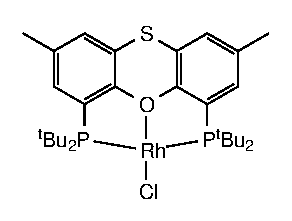
\includegraphics{../Structures/RhCl(StBu).eps}
%\end{center}
%\end{structure}

%7001, 7013%
This compound was synthesised similarly to [Rh(\tBusixantphos)Cl] using, \tButhixantphos{} (0.025 g, 0.048 mmol) and \ce{[Rh(coe)2Cl]_{n}} (0.021 g, 0.059 mmol).  The title compound was obtained as an air-sensitive brown solid in quantitative yield (0.032 g, 0.048 mmol, 100\%).  

\Phosphorusintro{C6D6}
\NMRRhP{46.5}{141.5}
\Protonintro{600}{C6D6}
\NMRcoupled{7.43}{d}{1.5}{\StBucH},
\NMRsinglet{6.39}{\StBuaH},
\NMRsinglet{1.81}{\StBugH},
\NMRcoupled{1.67}{vt}{13.6}{\StBuiH}.
\Carbonintro{150}{C6D6}
\NMRPC{157.4}{vt}{16.8}{\StBueC},
\NMRPC{134.0}{vt}{3.6}{\StBubC},
\NMRsinglet{133.7}{\StBucC},
\NMRsinglet{128.5}{\StBuaC},
\NMRPC{127.4}{vt}{8.1}{\StBufC},
\NMRPC{117.9}{vt}{7.6}{\StBudC},
\NMRPC{37.7}{vt}{9.2}{\StBuhC},
\NMRPC{30.9}{vt}{7.5}{\StBuiC},
\NMRsinglet{19.8}{\StBugC}.
HRMS calcd for \ce{C30H46OP2RhS} [M-Cl]$^+$ \emph{m/z} = 619.1794; found = 619.1795.


%%%%%%%%
%Rh(CtBu)Cl %
%%%%%%%%

\subsection*{[Rh(\tBuxantphosk)Cl]}

%\begin{structure}[h]
%\begin{center}
%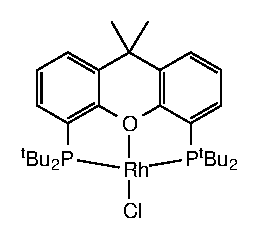
\includegraphics{../Structures/RhCl(CtBu).eps}
%\end{center}
%\end{structure}

%7012%
The compound was synthesised similarly to [Rh(\tBusixantphos)Cl] using \tBuxantphos{} (0.019 g, 0.038 mmol) and \ce{[Rh(coe)2Cl]_{n}} (0.016 g, 0.038 mmol).  A dark red solid was obtained in quantitative yield (0.024 g, 0.038 mmol, 98.9\%).  

\Phosphorusintro{C6D6}
\NMRRhP{47.7}{142.3}
\Protonintro{500}{C6D6}
\NMRcoupled{7.78}{d}{7.3}{\CtBucH},
\NMRcoupled{7.01}{d}{7.6}{\CtBuaH},
\NMRcoupled{6.80}{t}{7.7}{\CtBubH},
\NMRPH{1.68}{vt}{13.4}{\CtBujH},
\NMRsinglet{1.16}{\CtBuhH}.
\Carbonintro{125}{C6D6}
\NMRPC{158.9}{vt}{16.3}{\CtBueC},
\NMRsinglet{133.6}{\CtBucC},
\NMRPC{131.3}{vt}{6.23}{\CtBufC},
\NMRsinglet{127.7}{\CtBuaC},
\NMRPC{125.7}{vt}{12.0}{\CtBudC},
\NMRsinglet{123.8}{\CtBubC},
\NMRPC{37.6}{vt}{10.1}{\CtBuiC},
\NMRsinglet{32.5}{\CtBugC},
\NMRsinglet{33.8}{\CtBuhC},
\NMRPC{30.8}{vt}{7.7}{\CtBujC}.
HRMS calcd for \ce{C31H48OP2Rh} [M-Cl]$^+$ \emph{m/z} = 601.2230; found = 601.2222.


%%%%%%%%%%
% Rh(SitBu)Cl(H)2%
%%%%%%%%%%

\subsection*{(\emph{OC}-6-43)-\texorpdfstring{[Rh(\tBusixantphosk)Cl(H\ce{)2]}}R}

%\begin{structure}[h]
%\begin{center}
%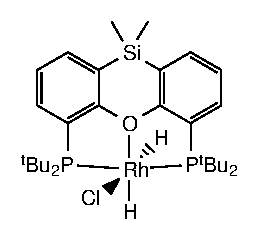
\includegraphics{../Structures/SitBuRhClH2.eps}
%\end{center}
%\end{structure}

%7007%
\ce{C6D6} (0.5 mL) was stirred vigorously under hydrogen for 10 mins, before using to dissolve [Rh(\tBusixantphos)Cl] (0.037 g, 0.057 mmol) in a Young's tap NMR tube.  Hydrogen was bubbled through the solution for 10 mins before sealing the tube under hydrogen.  After 48 hours removal of the solvent \emph{in vacuo} yielded the title compound as a brown solid in quantitative yield (0.037 g, 0.056 mmol).  

\Phosphorusintro{C6D6}
78.2 (ddd, \JRhP{} = 116.1, \JPH{} = 12.1, 2.7 Hz).
\Protonintro{600}{C6D6}
\NMRmultiplet{7.71}{\SitBucH},
\NMRcoupled{7.23}{dd}{7.1, 1.7}{\SitBuaH},
\NMRcoupled{6.93}{t}{7.4}{\SitBubH},
\NMRcoupled{1.75}{vt}{14.7}{\SitBuiH},
\NMRcoupled{1.29}{vt}{13.7}{\SitBuiH},
\NMRsinglet{0.17}{\SitBugH},
\NMRsinglet{0.10}{\SitBugH},
-16.92 (dtd, \JRhH{} = 22.7, \JPH{} = 13.5, \JHH{} 9.4, \ce{H-} \emph{trans} \ce{Cl-}),
-21.12 (dtd, \JRhH{} = 30.9, \JPH{} = 12.1, \JHH{} 9.2, \ce{H-} \emph{trans} \ce{O}).
\Carbonintro{150}{C6D6}
\NMRcoupled{165.6}{vt}{11.0}{\SitBueC},
\NMRsinglet{137.5}{\SitBucC},
\NMRsinglet{136.4}{\SitBuaC},
\NMRcoupled{126.5}{vt}{15.0}{\SitBudC},
\NMRcoupled{122.6}{vt}{4.6}{\SitBubC},
\NMRsinglet{122.0}{\SitBufC},
\NMRcoupled{38.4}{vt}{10.9}{\SitBuhC},
\NMRcoupled{36.7}{vtt}{20.8, 2.8}{\SitBuhC},
\NMRcoupled{33.5}{vt}{8.5}{\SitBuiC},
\NMRbsinglet{30.0}{\SitBuiC},
\NMRsinglet{-0.7}{\SitBugC},
\NMRsinglet{-0.9}{\SitBugC}.
HRMS calcd for \ce{C30H50OP2RhSi} [M-Cl]$^+$ \emph{m/z} = 619.2156; found = 619.2137.

%%%%%%%%%%
% Rh(StBu)Cl(H)2%
%%%%%%%%%%

\subsection*{(\emph{OC}-6-43)-\texorpdfstring{[Rh(\tButhixantphosk)Cl(H\ce{)2]}} R}

%\begin{structure}[h]
%\begin{center}
%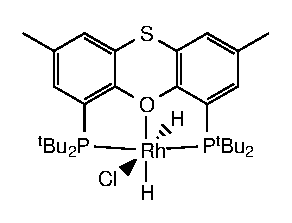
\includegraphics{../Structures/StBuRhClH2.eps}
%\end{center}
%\end{structure}

%7006%
The reaction was performed using the same method as the synthesis of [Rh(\tBusixantphos)\ce{Cl(H)2]}, using \tButhixantphos{} (0.034 g, 0.052 mmol).  NMR analysis after 48 hours showed the title compound as the only product.  The solvent was removed under reduced pressure, yielding the title compound as a brown solid in quantitative yield (0.034 g).  

\Phosphorusintro{C6D6}
77.8 (ddd, \JRhP{} = 117.8, \JPH{} = 11.9, 3.7).
\Protonintro{600}{C6D6}
\NMRcoupled{7.15}{d}{2.1}{\StBucH},
\NMRsinglet{6.51}{\StBuaH},
\NMRsinglet{1.85}{\StBugH},
\NMRcoupled{1.75}{vt}{14.6}{\StBuiH},
\NMRcoupled{1.29}{vt}{13.9}{\StBuiH},
-17.00 (dtd, \JRhH{} = 22.6, \JPH{} = 13.5, \JHH{} 9.4, \ce{H-} \emph{trans} \ce{Cl-}),
-21.13 (dtd, \JRhH{} = 30.5, \JPH{} = 12.4, \JHH{} 9.4, \ce{H-} \emph{trans} \ce{O}).
\Carbonintro{150}{C6D6}
\NMRcoupled{155.4}{vt}{13.8}{\StBueC},
\NMRcoupled{133.8}{vt}{4.6}{\StBubC},
\NMRsinglet{133.1}{\StBucC},
\NMRsinglet{129.1}{\StBuaC},
\NMRcoupled{126.7}{vt}{16.2}{\StBufC},
\NMRcoupled{120.2}{vt}{6.9}{\StBudC},
\NMRcoupled{38.3}{vt}{10.9}{\StBuhC},
\NMRcoupled{36.5}{vtt}{19.1, 2.5}{\StBuhC},
\NMRcoupled{33.2}{vt}{8.1}{\StBuiC},
\NMRbsinglet{30.1}{\StBuiC},
\NMRsinglet{20.1}{\StBugC}.

%%%%%%%%%%
%Rh(CtBu)Cl(H)2%
%%%%%%%%%%
 
\subsection*{(\emph{OC}-6-43)-\texorpdfstring{[Rh(\tBuxantphosk)Cl(H\ce{)2]}} R}

%\begin{structure}[h]
%\begin{center}
%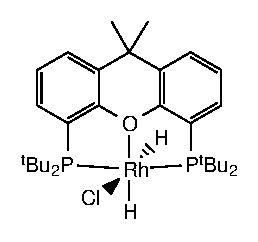
\includegraphics{../Structures/CtBuRhClH2.eps}
%\end{center}
%\end{structure}

%7005%
This reaction was performed using the same method as the synthesis of [Rh(\tBusixantphos)\ce{Cl(H)2]}, using [Rh(\tBuxantphos)Cl] (0.023 g, 0.036 mmol).  After 48 hours the solvent was removed in vacuo yielding the title compound as a brown solid in quantitative yield (0.023 g).

\Phosphorusintro{C6D6}
79.0 (ddd, \JRhP{} = 117.0, \JPH{} = 11.9, 5.2).
\Protonintro{600}{C6D6}
\NMRmultiplet{7.48}{\CtBucH},
\NMRcoupled{7.08}{d}{7.5}{\CtBuaH},
\NMRcoupled{6.88}{t}{7.6}{\CtBubH},
\NMRcoupled{1.77}{vt}{14.8}{\CtBujH},
\NMRcoupled{1.30}{vt}{13.7}{\CtBujH},
\NMRsinglet{1.25}{\CtBuhH},
\NMRsinglet{1.22}{\CtBuhH},
-17.04 (dtd, \JRhH{} = 22.8, \JPH{} = 13.4, \JHH{} 9.4, \ce{H-} \emph{trans} \ce{Cl-}),
-20.51 (dtd, \JRhH{} = 28.8, \JPH{} = 12.2, \JHH{} 9.4, \ce{H-} \emph{trans} \ce{O}).
\Carbonintro{150}{C6D6}
\NMRcoupled{156.2}{vt}{13.3}{\CtBueC},
\NMRsinglet{132.9}{\CtBuaC},
\NMRcoupled{132.4}{vt}{5.2}{\CtBufC}
\NMRcoupled{127.8}{vt}{8.1}{\CtBucC},
\NMRcoupled{125.1}{vt}{17.9}{\CtBudC},
\NMRcoupled{123.5}{vt}{4.6}{\CtBubC},
\NMRcoupled{38.1}{vt}{11.6}{\CtBuiC},
\NMRcoupled{36.5}{vtt}{19.1}{\CtBuiC},
\NMRsinglet{34.8}{\CtBugC},
\NMRcoupled{33.5}{vt}{7.5}{\CtBujC},
\NMRsinglet{32.4}{\CtBuhC},
\NMRsinglet{30.4}{\CtBuhC},
\NMRbsinglet{30.0}{\CtBujC}.

%%%%%%%%%%%%%
%% Rh(CtBu)Cl(H)2 + H%
%%%%%%%%%%%%%
%
%\subsection*{Attempted protonated of [Rh(\POP)Cl(H)2] using H2C(SO2CF3)2 (POP = \tBusixantphos, \tButhixantphos{} or \tBuxantphos)}
%
%%7008, 7009, 7010%
%\ce{H2C(SO2CF3)2} was weighed into a Young's tap NMR tube and placed under argon.  A d6-benzene (0.5 mL) solution of [Rh(\POP)Cl\ce{(H)2}] (0.023 g, 0.036 mmol)was added to the acid and the NMR tube was sealed under a hydrogen atmosphere.  The sample was analysed by NMR spectroscopy immediately.  
%
%\fixme{do I need to assign the spectra?}
%
%Tetrafluoroboric acid (3.7 \fixme{microL}) was added to a sample of [Rh(\POP)Cl\ce{(H)2}] in a Young's tap NMR tube under a hydrogen atmosphere.  The reaction was sealed and analysed by NMR spectroscopy.  

%%%%%%%%%%%
%Rh(SitBu)Cl(CO)2%
%%%%%%%%%%%

\subsection*{(\emph{TBPY}-5-33)-[Rh(\tBusixantphos-\dento{2}-\emph{P,P}\textprime)\ce{(CO)2}Cl]}

%\iupac{chlorodicarbonyl(\tBusixantphos-\dento{2}-\emph{P,P})rhodium(I)}}

%\begin{structure}[h]
%\begin{center}
%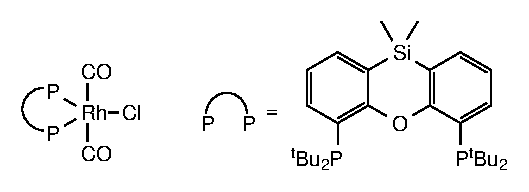
\includegraphics{../Structures/RhCl(SitBu)(CO)2.eps}
%\end{center}
%\end{structure}

[Rh(\tBusixantphos)Cl] (0.041 g, 0.063 mmol) was dissolved in \ce{C6D6} (0.5 mL) in a Young's tap NMR tube, under an argon atmosphere.  Carbon monoxide was bubble through the solution for 10 mins, before the tube was sealed under a carbon monoxide atmosphere.  After three days the reaction was complete by \phosphorus{} NMR spectroscopy.  The orange solution was decanted and the solvent was removed under reduced pressure, yielding the title complex as an orange solid (0.027 g, 0.038 mmol, 60\%). 

\Phosphorusintro{C6D6}
\NMRRhP{70.8}{120.0}.
\Protonintro{600}{C6D6}
\NMRmultiplet{7.69}{\SitBucH},
\NMRcoupled{7.32}{d}{6.8}{\SitBuaH},
\NMRcoupled{7.02}{t}{7.2}{\SitBubH},
\NMRcoupled{1.53}{vt}{14.0}{\SitBuiH},
\NMRsinglet{0.18}{\SitBugH}.
\Carbonintro{150}{C6D6}
\NMRcoupled{195.5}{dt}{84.4, 13.0}{Rh\emph{C}O}
\NMRcoupled{164.3}{vt}{8.1}{\SitBueC},
\NMRsinglet{138.1}{\SitBucC},
\NMRsinglet{136.5}{\SitBuaC},
\NMRcoupled{124.9}{vt}{24.2}{\SitBudC},
\NMRsinglet{123.2}{\SitBufC},
\NMRsinglet{122.4}{\SitBubC},
\NMRcoupled{38.4}{vt}{13.9}{\SitBuhC},
\NMRbsinglet{31.5}{\SitBuiC},
\NMRbsinglet{-1.5}{\SitBugC}.
HRMS calcd for \ce{C31H48O2P2RhSi} [M-COCl]$^+$ \emph{m/z} = 645.1948; found = 645.1959.


%%%%%%%%%%%
% Rh(StBu)Cl(CO)2%
%%%%%%%%%%%

\subsection*{(\emph{TBPY}-5-33)-[Rh(\tButhixantphos-\dento{2}-\emph{P,P}\textprime)\ce{(CO)2}Cl]}

%\begin{structure}[h]
%\begin{center}
%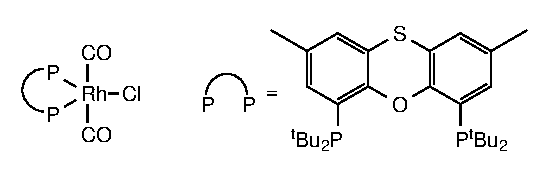
\includegraphics{../Structures/RhCl(StBu)(CO)2.eps}
%\end{center}
%\end{structure}

%7016%
This compound was synthesised similarly to [Rh(\tBusixantphos)\ce{(CO)2Cl}], using [Rh(\tButhixantphos)Cl] (0.032 g, 0.049 mmol) generating [Rh(\tButhixantphos)\ce{(CO)2Cl}] as a yellow solid, (0.025 g, 0.035 mmol, 72\%).  

\Phosphorusintro{C6D6}
\NMRRhP{69.3}{122.2}
\Protonintro{600}{C6D6}
\NMRsinglet{7.15}{Ar},
\NMRbsinglet{6.88}{Ar},
\NMRsinglet{1.88}{\StBugH},
\NMRbsinglet{1.52}{\StBuiH}.
\Carbonintro{150}{C6D6}
\NMRbsinglet{154.9}{\CtBueC},
\NMRsinglet{134.1}{Ar},
\NMRbsinglet{132.5}{Ar},
\NMRbsinglet{129.5}{Ar},
\NMRbsinglet{125.6}{Ar},
\NMRbsinglet{121.7}{Ar},
\NMRbsinglet{38.2}{\CtBuhC},
\NMRbsinglet{31.5}{\CtBuiC},
\NMRsinglet{20.3}{\CtBugC}.
HRMS calcd for \ce{C31H46O2P2RhS} [M-COCl]$^+$ \emph{m/z} = 647.1743; found = 647.1754.

%%%%%%%%%%%
%Rh(CtBu)Cl(CO)2 %
%%%%%%%%%%%

\subsection*{(\emph{TBPY}-5-33)-[Rh(\tButhixantphos-\dento{2}-\emph{P,P}\textprime)\ce{(CO)2}Cl]}

%\begin{structure}[h]
%\begin{center}
%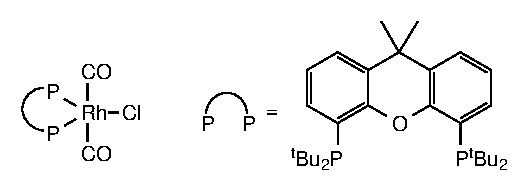
\includegraphics{../Structures/RhCl(CtBu)(CO)2.eps}
%\end{center}
%\end{structure}

This compound was synthesised similarly to [Rh(\tBusixantphos)\ce{(CO)2Cl}], using [Rh(\tBuxantphos)Cl] (0.024 g, 0.038 mmol) generating the title compound as a yellow solid, (0.018 g, 0.026 mmol, 67\%).  

\Phosphorusintro{C6D6}
\NMRRhP{71.6}{120.0}.
\Protonintro{600}{C6D6}
\NMRmultiplet{7.46}{\CtBucH},
7.15 (partially obscured by residual solvent peak, \CtBuaH),
\NMRcoupled{6.94}{t}{7.6}{\CtBubH},
\NMRcoupled{1.54}{vt}{13.8}{\CtBujH},
\NMRsinglet{1.24}{\CtBuhH}.
\Carbonintro{150}{C6D6}
\NMRcoupled{194.9}{dt}{84.4, 12.4}{Rh\emph{C}O},
\NMRcoupled{155.6}{vt}{10.4}{\CtBueC},
\NMRcoupled{133.4}{vt}{4.6}{\CtBufC},
\NMRsinglet{133.3}{\CtBucC},
\NMRsinglet{127.0}{\CtBuaC},
\NMRcoupled{123.9}{vt}{25.4}{\CtBudC},
\NMRcoupled{122.7}{vt}{5.3}{\CtBubC},
\NMRcoupled{38.1}{vt}{13.9}{\CtBuiC},
\NMRsinglet{35.3}{\CtBugC},
\NMRbsinglet{31.4}{\CtBujC},
\NMRbsinglet{29.5}{\CtBuhC}.
HRMS calcd for \ce{C32H48O2P2Rh} [M-COCl]$^+$ \emph{m/z} = 629.2179; found = 629.2186.


%%%%%%%%%%
% Rh(SitBu)ClO2 %
%%%%%%%%%%

\subsection*{\texorpdfstring{[Rh(\tBusixantphos)Cl(\hapto{2}-\ce{O2})]} R}

%\begin{structure}[h]
%\begin{center}
%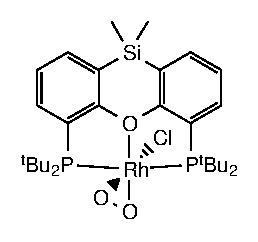
\includegraphics{../Structures/SitBuRhClO2.eps}
%\end{center}
%\end{structure}

Air was bubbled through an NMR sample of [Rh(\tBusixantphos)Cl] (0.050 g) in \ce{C6D6} for 10 mins.  After 24 hours at room temperature, NMR spectroscopy showed quantitative conversion to [Rh(\tBusixantphos)Cl(\hapto{2}-\ce{O2})].

\Phosphorusintro{C6D6}
\NMRRhP{39.4}{102.2}.
\Protonintro{600}{C6D6}
\NMRmultiplet{7.62}{\SitBucH},
\NMRcoupled{7.18}{dd}{7.0, 1.6}{\SitBuaH},
\NMRcoupled{6.89}{t}{7.2}{\SitBubH},
\NMRcoupled{1.87}{vt}{14.4}{\SitBuiH},
\NMRbsinglet{1.40}{\SitBuiH},
\NMRsinglet{0.19}{\SitBugH},
\NMRsinglet{0.01}{\SitBugH}.
\Carbonintro{150}{C6D6}
\NMRcoupled{166.7}{vt}{9.8}{\SitBueC},
\NMRsinglet{138.7}{\SitBucC},
\NMRsinglet{136.5}{\SitBuaC},
\NMRcoupled{124.6}{vt}{20.8}{\SitBudC},
\NMRsinglet{123.2}{\SitBufC},
\NMRcoupled{122.9}{vt}{4.7}{\SitBubC},
\NMRcoupled{39.1}{vt}{10.4}{\SitBuhC},
\NMRcoupled{38.9}{vt}{13.8}{\SitBuhC},
\NMRcoupled{33.4}{vt}{5.8}{\SitBuiC},
\NMRbsinglet{29.5}{\SitBuiC},
\NMRsinglet{0.8}{\SitBugC},
\NMRsinglet{-4.2}{\SitBugC},
HRMS calcd for \ce{C30H48O3P2RhSi} [M-Cl]$^+$ \emph{m/z} = 649.1898; found = 649.1917.

%%%%%%%%%%
% Rh(StBu)ClO2 %
%%%%%%%%%%

\subsection*{\texorpdfstring{[Rh(\tButhixantphos)Cl(\hapto{2}-\ce{O2})]} R}

%\begin{structure}[h]
%\begin{center}
%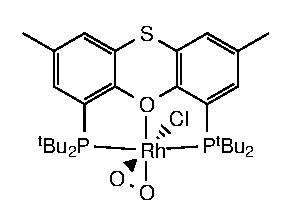
\includegraphics{../Structures/StBuRhClO2.eps}
%\end{center}
%\end{structure}

This compound was synthesised as for [Rh(\tBusixantphos)Cl(\hapto{2}-\ce{O2})] using [Rh(\tButhixantphos)Cl] (0.050 g).

\Phosphorusintro{C6D6}
\NMRRhP{39.0}{101.5}.
\Protonintro{500}{C6D6}
\NMRPH{7.07}{d}{2.2}{\StBucH},
\NMRsinglet{6.50}{\StBuaH},
\NMRcoupled{1.83}{vt}{14.5}{\StBuiH},
\NMRsinglet{1.79}{\StBugH},
\NMRbsinglet{1.44}{\StBuiH}.
\Carbonintro{125}{C6D6}
\NMRcoupled{155.9}{vt}{12.5}{\StBueC},
\NMRsinglet{134.6}{\StBucC},
\NMRcoupled{134.0}{vt}{5.3}{\StBubC},
\NMRsinglet{129.8}{\StBuaC},
\NMRcoupled{125.2}{vt}{19.7}{\StBudC},
\NMRcoupled{119.9}{vt}{7.2}{\StBufC},
\NMRcoupled{39.1}{vt}{10.6}{\StBuhC},
\NMRcoupled{38.9}{vt}{13.5}{\StBuhC},
\NMRcoupled{33.2}{vt}{5.5}{\StBuiC},
\NMRbsinglet{28.9}{\StBuiC},
\NMRsinglet{19.9}{\StBugC}.
HRMS calcd for \ce{C30H46O3P2Rh} [M-Cl]$^+$ \emph{m/z} = 651.1692; found = 651.1695.

%%%%%%%%%%
% Rh(CtBu)ClO2  %
%%%%%%%%%%

\subsection*{\texorpdfstring{[Rh(\tBuxantphos)Cl(\hapto{2}-\ce{O2})]} R}

%\begin{structure}[h]
%\begin{center}
%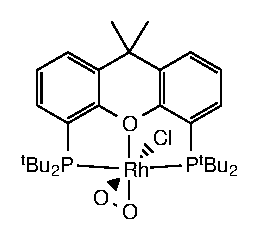
\includegraphics{../Structures/CtBuRhClO2.eps}
%\end{center}
%\end{structure}

This compound was synthesised as for [Rh(\tBusixantphos)Cl(\hapto{2}-\ce{O2})] using [Rh(\tBuxantphos)Cl] (0.050 g).

\begin{sloppypar}
\Phosphorusintro{C6D6}
\NMRRhP{40.5}{100.7}
\Protonintro{600}{C6D6}
\NMRmultiplet{7.40}{\CtBucH},
\NMRcoupled{7.08}{d}{7.5}{\CtBuaH},
\NMRcoupled{6.87}{t}{7.7}{\CtBubH},
\NMRcoupled{1.83}{vt}{14.4}{\CtBujH},
\NMRbsinglet{1.43}{\CtBujH},
\NMRsinglet{1.32}{\CtBuhH},
\NMRsinglet{1.00}{\CtBuhH}.
\Carbonintro{150}{C6D6}
\NMRcoupled{157.3}{vt}{11.5}{\CtBueC},
\NMRsinglet{133.9}{\CtBucC},
\NMRcoupled{133.1}{vt}{5.8}{\CtBufC},
\NMRsinglet{127.4}{\CtBuaC},
\NMRcoupled{123.9}{vt}{4.7}{\CtBubC},
\NMRcoupled{123.3}{vt}{21.6}{\CtBudC},
\NMRcoupled{38.9}{vt}{11.0}{\CtBuiC},
\NMRcoupled{38.7}{vt}{14.0}{\CtBuiC},
\NMRsinglet{35.5}{\CtBuhC},
\NMRsinglet{34.7}{\CtBugC},
\NMRcoupled{33.3}{vt}{5.8}{\CtBujC},
\NMRbsinglet{29.0}{\CtBujC},
\NMRsinglet{24.2}{\CtBuhC}.
HRMS calcd for \ce{C31H48O3P2Rh} [M-Cl]$^+$ \emph{m/z} = 633.2128; found = 633.2140.
\end{sloppypar}

\subsection*{Reaction of [Rh(\tBusixantphos)Cl] with \texorpdfstring{\ce{ONMe3}} O}

%6041

In a glovebox, solid \ce{ONMe3} (0.004 g, 0.05 mmol) was added to an NMR tube containing a \ce{CD2Cl2} solution of [Rh(\tBusixantphos)Cl] (0.035 g, 0.05 mmol).  The NMR tube was sealed with a J. Young tap.  By \phosphorus{} NMR spectroscopy the mixture contained uncoordinated \tBusixantphos{} (18.6\%), \tBusixantphos{} oxide (12.5\%) and [Rh(\tBusixantphos)Cl(\hapto{2}-\ce{O2})] (68.9\%).  After four days the reaction contained uncoordinated \tBusixantphos{} (6.1\%), \tBusixantphos{} oxide (5.3\%), [Rh(\tBusixantphos)Cl(\hapto{2}-\ce{O2})] (36.7\%),  [Rh(\tBusixantphos)Cl] (46.2\%) and an unidentified species possibly [Rh(\tBusixantphos)\ce{Cl2}(OH)] (5.8\%).

\subsubsection{[Rh(\tBusixantphos)\ce{Cl2}(OH)]}

\Phosphorusintro{CD2Cl2}
\NMRRhP{70.5}{114.1}
%\fixme{values from 6041C}

\subsection*{Reaction of [Rh(\tButhixantphos)Cl] with \texorpdfstring{\ce{ONMe3}} O}

In a glovebox, solid \ce{ONMe3} (0.008 g, 0.11 mmol) was added to an NMR tube containing a \ce{C6D6} solution of [Rh(\tButhixantphos)Cl] (0.066 g, 0.10 mmol).  The NMR tube was sealed with a J. Young tap.  Solid was evident in the NMR tube so the solvent was removed \emph{in vacuo} and replaced with \ce{CD2Cl2}.  By \phosphorus{} NMR the mixture contained uncoordinated \tButhixantphos{} (22.9\%), [Rh(\tButhixantphosk)Cl(\hapto{2}-\ce{O2})] (8.6\%), [Rh(\tButhixantphosk)Cl] (64.4\%) and a new compound proposed as [Rh(\tButhixantphosk)Cl(O)] (7.1\%).

\subsubsection{[Rh(\tButhixantphosk)Cl(O)]}

\Phosphorusintro{CD2Cl2}
\NMRRhP{40.9}{90.4}.

After 10 days no starting material remained and the reaction mixture contained [Rh(\tButhixantphosk)Cl(\hapto{2}-\ce{O2})] (66.7\%), [(\tButhixantphos)H\ce{]+} (14.2\%), \tButhixantphos{} (5.3\%) and a new complex proposed as [Rh(\tButhixantphos)\-\ce{Cl2}(OH)].

\subsubsection{[Rh(\tButhixantphos)\ce{Cl2}(OH)]}

\Phosphorusintro{CD2Cl2}
\NMRRhP{74.1}{116.3}.

\subsection*{Reaction of [Rh(\tBuxantphos)Cl] with \texorpdfstring{\ce{ONMe3}} O}

Solid \ce{ONMe3} (0.007 g, 0.088 mmol) was added to a solution of [Rh(\tBuxantphos)Cl] (0.056 g, 0.088 mmol) in \ce{CD2Cl2} at -78\degC{}.  The NMR tube was sealed with a J. Young tap, and immediately transferred to an NMR spectrometer at -80\degC.  The reaction contained unreacted [Rh(\tBuxantphos)Cl] (85.7\%) and [Rh(\tBuxantphos)Cl(\hapto{2}-\ce{O2})] (14.3\%).  Upon warming to room temperature over 24 hours the reaction mixture contained [Rh(\tBuxantphos)Cl] (25.4\%), [Rh(\tBuxantphos)Cl(\hapto{2}-\ce{O2})] (70.5\%), and a new set of peaks proposed as [Rh(\tBuxantphos)Cl(O)] (4.2\%).

\subsubsection{[Rh(\tBuxantphos)Cl(O)]}

\Phosphorusintro{CD2Cl2}
\NMRRhP{42.6}{90.4}.

After 14 days at room temperature the reaction mixture contained [Rh(\tBuxantphos)Cl(O)] (42.8\%), [Rh(\tBuxantphos)Cl(\hapto{2}-\ce{O2})] (49.9\%) and a new complex proposed as [Rh(\tBuxantphos)\ce{Cl2}(OH)] (7.3\%).

\subsubsection{[Rh(\tBuxantphos)\ce{Cl2}(OH)]}

\Phosphorusintro{CD2Cl2}
\NMRRhP{75.1}{116.3}

\section{Platinum Complexes}
\label{section:experimental:platinum}

%%%%%%
% PtSPh %
%%%%%%

\subsection*{1:1 Reaction of \Phthixantphos{} with [Pt(nb\ce{)3}]}

A solution of \Phthixantphos{} (0.020 g, 0.035 mmol) in \ce{C6D6} was added to an NMR tube containing tris(norbornene)platinum (0.017 g, 0.035 mmol).  Immediate \proton{} and \phosphorus{} NMR spectroscopy showed [Pt(nb)(\Phthixantphos)] (39.6\%) and [Pt(\Phthixantphos\ce{)2}] (60.4\%).  No change was observed in the ratio over 7 days.   

\subsubsection{[Pt(\Phthixantphos)(nb)]}

\Phosphorusintro{C6D6}
\NMRPPt{20.0}{3470}.
%\fixme{more data}

\subsection*{\texorpdfstring{[Pt(\Phthixantphos\ce{)2}]} P}

A solution of \Phthixantphos{} (0.200 g, 0.35 mmol) in toluene (5 mL) was added to tris(norbornene)platinum (0.084 g, 0.18 mmol) in toluene (5 mL).  The reaction was stirred for one hour before removing the solvent under reduced pressure.  The yellow powder was purified by recrystallisation from a mixture of toluene and diethyl ether yielding the title compound as a yellow microcrystalline solid (0.066 g, 14\%).  Single X-ray quality crystals were grown by inwards diffusion of diethyl ether into a dichloromethane solution of the complex over three days.  

%\fixme{structure}

Data at -80\degC:
\Phosphorusintro{CD2Cl2}
\NMRcoupled{-2.4}{t}{55.0, \JPtP~=~3976}{},
\NMRcoupled{-6.2}{t}{55.0, \JPtP{} = 3864}{}.
\Protonintro{300}{CD2Cl2}
\NMRmultiplet{5.7-7.4}{Ar}.
HRMS calcd for \ce{C72H52O2P4S2Pt} \ce{[M]+} m/z = 1330.2002; found = 1330.1986.

%%%%%%%%%
% PtSPhC2H4 % 
%%%%%%%%%
\subsection*{Reaction of \Phthixantphos{} with \texorpdfstring{\ce{[Pt(C2H4)3]}} P}

A solution of \Phthixantphos{} (0.017 g, 0.029 mmol) in \ce{C6D6} was added to an NMR tube containing tris(ethene)platinum (0.008 g, 0.029 mmol).  The reaction became orange after 10 minutes.  By \phosphorus{} NMR analysis [Pt(\Phthixantphos\ce{)2}] was the major product (93 \%) with a small amount of [Pt\ce{(C2H4)}(\Phthixantphos)] (7\%) as a minor component.  

\subsubsection{[Pt\ce{(C2H4)}(\Phthixantphos)]}

\Phosphorusintro{C6D6}
\NMRPPt{20.9}{3659}.
\Protonintro{300}{C6D6}
2.29 (s, \JPtH{} = 61.0 Hz, \ce{C=C-H}).
 
\subsection*{Reaction of \tButhixantphos{} with \texorpdfstring{[Pt(nb\ce{)3}]} P} 

In a glovebox, \tButhixantphos{} (0.057 g, 0.110 mmol) in \ce{C6D6} (0.5 mL) was added to a J. Young's tap NMR tube containing [Pt(nb\ce{)3}] (0.053 g, 0.110 mmol).  The NMR tube was closed under a nitrogen atmosphere and the reaction was heated to 60 \degC{} until the reaction was deemed complete by the absence of \tButhixantphos{} from the \phosphorus{} and \proton{} NMR spectra (4-6 days).  At this stage, \proton{}, \carbon{} and \phosphorus{} NMR analysis was carried out to characterise [Pt(\tButhixantphos)(nb)] complex (39.2\%).  The solution was filtered through a plug of diatomaceous earth washing through with toluene (2 x 1 mL).  The solvent was removed under reduced pressure for one hour leaving [Pt(\tButhixantphos)] as a brown expanded oil (0.073 g, 93\%).

\begin{structure}[h]
\begin{center}
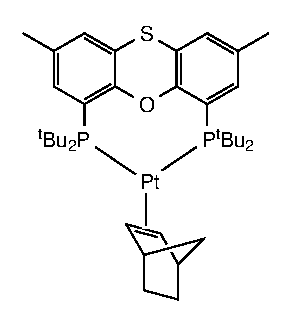
\includegraphics{../Structures/StBuPlatinumnorbornene.eps}
\end{center}
\end{structure}

\Phosphorusintro{C6D6}
\NMRPPt{55.6}{3612}
\Protonintro{600}{C6D6}
\NMRsinglet{7.61}{\StBucH},
\NMRsinglet{6.95}{\StBuaH},
\NMRsinglet{3.12}{nb CH},
\NMRPtH{2.37}{bs}{1}{67.8}{nb =C\emph{H}},
\NMRsinglet{1.96}{\StBugH},
\NMRobscuredH{1.93}{COSY}{2H}{nb C\emph{H}\sub{2}},
\NMRmultiplet{1.42-1.56}{\StBuiH},
\NMRobscuredH{1.32}{COSY}{3H}{nb C\emph{H}\sub{2}, bridge \ce{CH2}},
\NMRHH{0.62}{d}{15.3}{1H, nb bridge \ce{CH2}}.
\Carbonintro{150}{C6D6}
\NMRPC{158.9}{vt}{9.8}{\StBueC},
\NMRPtC{135.4}{s}{2}{26.6}{\StBucC},
\NMRbsinglet{130.9}{\StBubC},
\NMRbsinglet{130.7}{\StBuaC},
\NMRPC{127.6}{vt}{5.8}{\StBufC},
\NMRbsinglet{125.9}{\StBudC},
\NMRPtC{51.9}{bs}{1}{343.9}{nb =\emph{C}H},
\NMRsinglet{44.9}{nb \emph{C}H},
\NMRmultiplet{38.5}{\StBuhC},
\NMRobscuredC{38.0-38.5}{HSQC}{nb bridge \emph{C}\ce{H2}},
\NMRbsinglet{31.7}{\StBuiC},
\NMRPtC{31.4}{bs}{3}{61.4}{nb \emph{C}\ce{H2}},
\NMRsinglet{20.7}{\StBugC}.

\begin{structure}[h]
\begin{center}
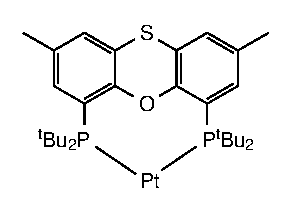
\includegraphics{../Structures/StBuPlatinum.eps}
\end{center}
\end{structure}

\Phosphorusintro{C6D6}
\NMRPPt{78.6}{4809.5}
\Protonintro{600}{C6D6}
\NMRPH{7.32}{d}{1.8}{\StBucH},
\NMRsinglet{6.87}{\StBuaH},
\NMRsinglet{1.95}{\StBugH},
\NMRPH{1.52}{vt}{13.8}{\StBuiH}.
\Carbonintro{150}{C6D6}
\NMRPC{155.9}{vt}{10.4}{\StBueC},
\NMRsinglet{133.3}{\StBucC},
\NMRPC{132.1}{vt}{5.2}{\StBubC},
\NMRsinglet{128.8}{\StBuaC},
\NMRPC{126.6}{vt}{28.9}{\StBudC},
\NMRPC{126.1}{vt}{5.8}{\StBufC},
\NMRPC{37.8}{vt}{15}{\StBuhC},
\NMRPC{31.7}{vt}{10.4}{\StBuiC},
\NMRsinglet{20.5}{\StBugC}.
HRMS calcd for \ce{C30H47OP2PtS} \ce{[M+H]+} m/z = 711.2438; found = 711.2450.

%%%%%%%
\subsection*{Reaction of \tBusixantphos{} with \texorpdfstring{[Pt(nb\ce{)3}]} P}

A solution of \tBusixantphos{} (0.19 g, 0.37 mmol) in \ce{C6D6} (0.5 mL) was added to \ce{[Pt(nb)3]} (0.018 g, 0.37 mmol) in a J. Young's tap NMR tube.  After 24 hours at 60\degC{} the \phosphorus{} NMR spectrum showed a mixture of unreacted \tBusixantphos{} (75.0\%), [Pt(\tBusixantphos)] (15.8\%), and [Pt(\tBusixantphos)(nb)] (9.2\%).  After five days at 60\degC{} the reaction mixture contained unreacted \tBusixantphos{} (11.1\%), [Pt(\tBusixantphos)] (32.5\%), [Pt(\tBusixantphos)(nb)] (24.1\%) and an unidentified Pt(II) species (18.2\%).  

\subsubsection*{[Pt(\tBusixantphos)]}

\Phosphorusintro{C6D6}
\NMRPPt{79.5}{4826.6}

\subsubsection*{[Pt(\tBusixantphos)(nb)]}

\Phosphorusintro{C6D6}
\NMRPPt{59.3}{3571.8}

\subsubsection*{Pt(II) \tBusixantphos{} species}

\Phosphorusintro{C6D6}
\NMRPPt{34.7}{2676.9}

%%%%%%%%
% PtCtBuH X %
%%%%%%%%
\subsection*{[Pt(\tBuxantphos)H]X}

%\fixme{include a counterion in heading}
%\fixme{include a structure}

A solution of \tBuxantphos{} (0.016 g, 0.032 mmol) in \ce{C6D6} (0.5 mL) was added to tris-(norbornene)-platinum (0.015 g, 0.032 mmol) in an Young's tap NMR tube.  The tube was closed under argon and heated to 60 \degC{} overnight.  After 24 hours no free ligand remained and the major product is proposed as [Pt(\tBuxantphosk)H]X.  After 7 days at room temperature small yellow crystals had formed.  The solution was decanted and the product was isolated (0.020 g).  

\begin{sloppypar}
\Phosphorusintro{C6D6}
\NMRPPt{46.7}{3246}
\Protonintro{600}{C6D6}
\NMRmultiplet{7.43}{\CtBucH},
\NMRcoupled{7.11}{d}{7.5}{\CtBuaH},
\NMRcoupled{6.84}{t}{7.6}{\CtBubH},
\NMRbsinglet{1.7}{\CtBuhH},
\NMRbsinglet{1.5}{\CtBujH},
\NMRcoupledPtH{-18.49}{t}{13.1}{1}{1107}{\ce{Pt-H}}.
\Carbonintro{150}{C6D6}
\NMRcoupled{158.6}{vt}{8.0}{\CtBueC},
\NMRcoupled{138.4}{vt}{4.1}{\CtBufC},
\NMRsinglet{132.1}{\CtBucC},
\NMRcoupled{124.8}{vtd}{39.3, 2.9}{\CtBudC},
\NMRsinglet{125.8}{\CtBuaC},
\NMRcoupled{121.8}{vt}{5.7}{\CtBubC},
\NMRcoupled{38.0}{vt}{17.5}{\CtBuiC},
\NMRsinglet{36.7}{\CtBugC},
\NMRbsinglet{30.7}{\CtBujC}.
HRMS calcd for \ce{C31H49OP2Pt} \ce{[M-X]+} m/z = 689.2858; found = 689.2864.
\end{sloppypar}

%%%%%%%%%%%
% Pt(COD)2 + StBu %
%%%%%%%%%%%
\subsection*{Reaction of \tButhixantphos{} with \texorpdfstring{[Pt(cod\ce{)2]}} P}

A solution of \tButhixantphos{} (0.026 g, 0.050 mmol) in \ce{C6D6} (0.3 mL) was added to a solution of bis-(1,5-cyclooctadiene)platinum (0.020 g, 0.050 mmol) in \ce{C6D6} (0.3 mL).  The NMR tube was closed with a septum and the reaction was followed by \proton{} and \phosphorus{} NMR spectroscopy.  After 48 hrs at room temperature the reaction had become black and contained 72 \% unreacted \tButhixantphos{} with the remainder being [Pt(\tButhixantphos)].  The reaction was heated to 40 \degC{} for 24 hours, then 60 \degC{} for 24 hours, but no further reaction was observed.  

\subsection*{Reaction of \tBusixantphos{} with \texorpdfstring{[Pt\ce{(C2H4)3}]} P}

\ce{C6D6} (0.5 mL) which had been previously dried and degassed then stored under Ar, was sparged by bubbling ethene through the liquid for 10 mins, then stirring vigorously under an ethene atmosphere for a further 10 mins.  [Pt(cod\ce{)2}] (0.026 g, 0.063 mmol) was placed under ethene and 0.03 mL of the \ce{C6D6} was added.  The solution was stirred vigorously for 30 mins to ensure complete conversion to [Pt\ce{(C2H4)3}].  \tBuSixantphos(0.032 g, 0.063 mmol) was placed in a Young's tap NMR tube under an ethene atmosphere and dissolved in the remaining \ce{C6D6}.  The [Pt\ce{(C2H4)3}] solution was added to the NMR tube, which was closed under ethene and shaken to ensure mixing of the solutions.  After four hours at room temperature [Pt(\tBusixantphos)(\ce{C2H4})] (11.1\%) had been produced.  The reaction did not proceed further.

\Phosphorusintro{C6D6}
\NMRPPt{53.7}{3499}.

%%%%%%%%%
% PtStBuC2H4 %
%%%%%%%%%
\subsection*{\texorpdfstring{[Pt(\tButhixantphos)\ce{(C2H4)}]} P}

%\begin{structure}[h]
%\begin{center}
%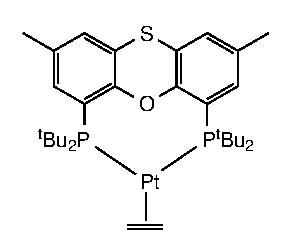
\includegraphics{../Structures/StBuPlatinumethene.eps}
%\end{center}
%\end{structure}

%Bis-(1,5-cyclooctadiene)platinum (0.109 g, 0.265 mmol) was weighed into a Schlenk tube and cooled in an ice bath before placing under an ethene atmosphere. Toluene, was stirred vigorously under an ethene atmosphere for 30 mins before adding 5 mL to the Schlenk tube.  The reaction was stirred for 30 mins to ensure complete conversion to [Pt(\ce{C2H4)3}] before adding to a solution of \tButhixantphos{} (0.137 g, 0.265 mmol) in the ethene sparged toluene (5 mL).  The reaction mixture was sealed under ethene and stirred at room temperature for 48 hours.  The toluene was removed under vacuum and the resulting brown solid was taken up in \ce{C6D6}, under ethene for NMR analysis.

\ce{C6D6} (0.5 mL) which had been previously dried and degassed then stored under Ar, was sparged by bubbling ethene through the liquid for 10 mins, then stirring vigorously under an ethene atmosphere for a further 10 mins.  Bis-(1,5-cyclooctadiene)platinum (0.032 g, 0.078 mmol) was placed under ethene and 0.03 mL of the \ce{C6D6} was added.  The solution was stirred vigorously for 30 mins to ensure complete conversion to [Pt\ce{(C2H4)3}].  \tBuThixantphos(0.040 g, 0.077 mmol) was placed in a Young's tap NMR tube under an ethene atmosphere and dissolved in the remaining \ce{C6D6}.  The [Pt\ce{(C2H4)3}] solution was added to the NMR tube, which was closed under ethene and shaken to ensure mixing of the solutions.  After 48 hours at room temperature the only product was [Pt(\tButhixantphos)(\ce{C2H4})] (100 \% by NMR).  

\Phosphorusintro{C6D6}
\NMRPPt{55.7}{3899}
\Protonintro{600}{C6D6}
\NMRsinglet{7.63}{\StBucH},
\NMRsinglet{6.96}{\StBuaH},
\NMRPtH{2.50}{bs}{2}{59.5}{\ce{C=C\emph{H\sub{2}}}},
\NMRsinglet{1.97}{\StBugH},
\NMRmultiplet{1.38-1.40}{\StBuiH}.
\Carbonintro{150}{C6D6}
\NMRbsinglet{158.7}{\StBueC},
\NMRPtC{135.3}{s}{4}{29.5}{\StBucC},
\NMRbsinglet{131.0}{\StBubC},
\NMRbsinglet{130.5}{\StBuaC},
\NMRPC{128.5}{vt}{5.8}{\StBufC},
\NMRbsinglet{125.7}{\StBudC},
\NMRmultiplet{38.7}{\StBuhC},
\NMRPtC{34.2}{bs}{1}{223.2}{\ce{C=C}}
\NMRbsinglet{31.6}{\StBuiC},
\NMRsinglet{20.7}{\StBugC}.

%%%%%%%%%
%PtCtBu(C2H4)%
%%%%%%%%%
%7036

\subsection*{Reaction of \tBuxantphos{} with \texorpdfstring{[Pt\ce{(C2H4)3}]} P}

%\begin{structure}[h]
%\begin{center}
%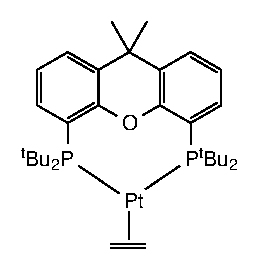
\includegraphics{../Structures/CtBuPtethene.eps}
%\end{center}
%\end{structure}

\ce{C6D6} (0.5 mL) which had been previously dried and degassed then stored under Ar, was sparged by bubbling ethene through the liquid for 10 mins, then stirring vigorously under an ethene atmosphere for a further 10 mins.  [Pt(cod\ce{)2}] (0.015 g, 0.036 mmol) was placed under ethene and 0.03 mL of the \ce{C6D6} was added.  The solution was stirred vigorously for 30 mins to ensure complete conversion to [Pt\ce{(C2H4)3}].  \tBuXantphos(0.018 g, 0.036 mmol) was placed in a Young's tap NMR tube under an ethene atmosphere and dissolved in the remaining \ce{C6D6}.  The [Pt\ce{(C2H4)3}] solution was added to the NMR tube, which was closed under ethene and shaken to ensure mixing of the solutions.  Both [Pt(\tBuxantphos)\ce{(C2H4)}] (41.7\%) and [Pt(\tBuxantphos)H]X (8.6\%)) were evident after four hours at room temperature.  After five days [Pt(\tBuxantphos)H]X was the only phosphorus containing compound in solution.

\subsubsection*{[Pt(\tBuxantphos)\ce{(C2H4)}]}

\begin{sloppypar}
\Phosphorusintro{C6D6}
\NMRPPt{53.4}{3878}
\Protonintro{600}{C6D6}
\NMRcoupled{7.79}{d}{6.8}{\CtBucH},
\NMRcoupled{7.09}{dd}{7.6, 1.1}{\CtBuaH},
\NMRcoupled{6.87}{t}{7.7}{\CtBubH},
\NMRPtH{2.52}{bs}{2}{58.0}{\ce{C=C\emph{H\sub{2}}}},
\NMRsinglet{1.43}{\CtBuhH},
\NMRcoupled{1.42}{d}{13.0}{\CtBujH}.
\Carbonintro{150}{C6D6}
\NMRmultiplet{161.0}{\CtBueC},
\NMRsinglet{138.4}{\CtBufC},
\NMRPtC{133.6}{s}{4}{28.1}{\CtBucC},
\NMRsinglet{124.6}{\CtBuaC},
\NMRmultiplet{124.1}{\CtBudC},
\NMRsinglet{121.2}{\CtBubC},
\NMRcoupled{38.4}{vt}{18.5, \twoJPtC = 34.1}{\CtBuiC},
\NMRsinglet{37.4}{\CtBugC},
\NMRcoupled{31.6}{vt}{8.1, \threeJPtC = 17.3}{\CtBujC}
\NMRsinglet{25.6}{\CtBuhC}.
\end{sloppypar}

%%%%%%%
%PtStBuO2%
%%%%%%%
\subsection*{\texorpdfstring{[Pt(\tButhixantphos)(\hapto{2}-\ce{O2})]} P}

%\begin{structure}[h]
%\begin{center}
%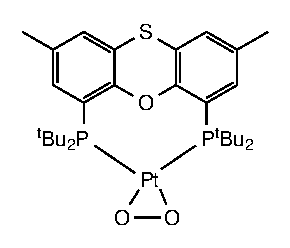
\includegraphics{../Structures/StBuPtO2.eps}
%\end{center}
%\end{structure}

A solution of \tButhixantphos{} (0.117 g, 0.23 mmol) in toluene (1 mL) was added to a Schlenk tube containing tris-(norbornene)platinum (0.108 g, 0.023 mmol) in toluene (3 mL).  The reaction was stirred at 40 \degC{} for 3 days.  The solvent was reduced in vacuo and the reaction mixture was placed under air.  The title compound was isolated by cooling the reaction mixture for two weeks at -20 \degC{} forming [Pt(\tButhixantphos)(\hapto{2}-\ce{O2)}] as a pale peach solid (0.109 g, 65\%).  X-ray quality crystals were grown by slow diffusion of air into a \ce{C6D6} solution of [Pt(\tButhixantphos)].

\Phosphorusintro{CD2Cl2}
\NMRPPt{38.4}{4488}
\Protonintro{600}{CD2Cl2}
\NMRcoupled{7.59}{dd}{5.9, 1.0}{a},
\NMRsinglet{7.32}{c},
\NMRsinglet{2.34}{g},
\NMRPH{1.43}{d}{14.4}{C(Ar)\ce{C\emph{H}3}}.
\Carbonintro{125}{CD2Cl2}
\NMRbsinglet{156.6}{\emph{C}O},
\NMRPtC{133.8}{s}{2}{37.9}{PC(Ar)\emph{C}H},
\NMRPC{133.1}{d}{5.3}{\emph{C}(Ar)\ce{CH3}},
\NMRbsinglet{131.7}{SCC\emph{C}(\ce{CH3})},
\NMRsinglet{128.5}{\emph{C}S},
\NMRPC{119.3}{d}{27.8}{P\emph{C}(Ar)},
\NMRPC{39.3}{d}{23.5}{P\emph{C}\ce{CH3}},
\NMRPC{31.2}{d}{5.3}{PC\emph{C}\ce{H3}},
\NMRsinglet{21.2}{C(Ar)\emph{C}\ce{H3}}.
HRMS calcd for \ce{C30H47O3P2PtS} [M+\ce{H]+} m/z = 743.2326; found = 743.2291.

%%%%%%%%%%%%%%%%
%Reactions of Pt(C2H4)StBu %
%%%%%%%%%%%%%%%%
\subsection*{Reaction of \texorpdfstring{[Pt(\tButhixantphos)(\ce{C2H4})]} P with Air}
%3021
Air was bubbled through a solution of [Pt(\tButhixantphos)(\ce{C2H4})] (0.020 g, 0.027 mmol) in \ce{C6D6} (0.4 mL) for a total of 10 mins.  The sample was sealed under air with a septum and analysed by NMR spectroscopy immediately.  [Pt(\tButhixantphos)(\hapto{2}-\ce{O2})] was produced in quantitative yield by NMR spectroscopy.  

\subsection*{Reaction of \texorpdfstring{[Pt(\tButhixantphos)(\ce{C2H4})]} P with argon}
%3022
Argon was bubbled through a solution of [Pt(\tButhixantphos)(\ce{C2H4})] (0.020 g, 0.027 mmol) in \ce{C6D6} (0.4 mL) for 10 mins.  The sample was sealed under argon and NMR analysis showed slight conversion to [Pt(\tButhixantphos)].  

%%%%%%%%
% Metallated  %
%%%%%%%%
\subsection*{Reaction of \texorpdfstring{[Pt(\tButhixantphos)(\hapto{2}-\ce{O2})]} P with CO}

Carbon monoxide was bubbled through a solution of [Pt(\tButhixantphos)(\hapto{2}-\ce{O2)}] (0.032 g, 0.043 mmol) in \ce{CD2Cl2} (0.4 mL) for 10 mins.  The reaction was followed by NMR spectroscopy and no further changes were observed after 7 days.  The solution was passed through an alumina plug (washing with 3 x 1 mL \ce{CH2Cl2}) and the solvent removed \emph{in vacuo} to give the metallated complex shown below as a brown solid (0.010 g, 32\%).  

Reaction with \ce{^{13}CO}:
[Pt(\tButhixantphos)(\hapto{2}-\ce{O2)}] (0.030 g, 0.040 mmol) was dissolved in \ce{CD2Cl2} and transferred to an NMR tube and sealed with a septum.  The sample was frozen in liquid nitrogen and attached by cannula to a solid potassium hydroxide trap, which in turn was attached to a sample vial containing \carbon{}-sodium formate.  The system was placed under vacuum, using syringes attached to both the NMR tube and the sample vial.  The system was closed under vacuum and the NMR tube was transferred to a dry ice/acetone bath and allowed to melt.  The vacuum syringe on the NMR tube was replaced with a gas-tight syringe to collect any excess carbon monoxide that may be produced.  Conc. sulfuric acid (1 mL) was added dropwise into the sample vial containing sodium formate producing rapid bubbling.  The set-up was left until the bubbling had mostly abated (approx. 10 mins).  All syringes and the cannula were removed from the sample vial and the septum was secured with Parafilm.  No unexpected differences were observed in the NMR spectra.  

\begin{structure}[h]
\begin{center}
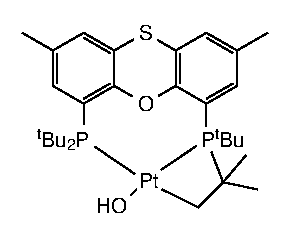
\includegraphics{../Structures/Metallated.eps}
\end{center}
\end{structure}

\Phosphorusintro{CD2Cl2}
\NMRPtwoPt{38.2}{s}{1794}{\ce{P}-\textsuperscript{t}\ce{Bu2}},
\NMRPtwoPt{$-$49.6}{s}{3943}{\ce{PCCPt}}.
\Protonintro{600}{CD2Cl2}
\NMRPH{7.60}{d}{3.8}{\ce{c2}},
\NMRsinglet{7.25}{\ce{a1}},
\NMRsinglet{7.16}{\ce{a2}},
\NMRPH{6.95}{d}{6.5}{\ce{c1}},
\NMRsinglet{2.34}{\ce{g1}},
\NMRsinglet{2.32}{\ce{g2}},
\NMRPH{1.71}{d}{12.9}{\ce{i3}},
\NMRcoupled{1.41}{d}{15.9}{\ce{k}},
\NMRcoupled{1.36}{d}{14.9}{l},
\NMRPH{1.34}{d}{13.2}{\ce{i2}},
\NMRmultiplet{1.2-1.5, obscured}{m},
\NMRPH{1.03}{d}{15.0}{\ce{i1}}.
\Carbonintro{150}{CD2Cl2},
\NMRPC{157.1}{d}{9.0}{\ce{e2}},
\NMRPC{153.9}{d}{4.3}{\ce{e1}},
\NMRPC{134.2}{d}{3.2}{\ce{c2}},
\NMRPC{133.8}{d}{6.3}{\ce{b1}},
\NMRPC{133.4}{d}{3.2}{\ce{b2}},
\NMRsinglet{132.8}{\ce{c1}},
\NMRPC{130.5}{d}{1.6}{\ce{a1}},
\NMRPC{129.6}{d}{1.6}{\ce{a2}},
\NMRPC{128.5}{dd}{4.2, 1.6}{\ce{f1}},
\NMRPC{124.0}{d}{4.3}{\ce{f2}},
\NMRPC{121.3}{d}{13.8}{\ce{d2}},
\NMRPC{116.6}{dd}{30.7, 1.6}{\ce{d1}},
\NMRPC{46.7}{d}{37.6}{j}
\NMRPC{40.8}{d}{10.1}{\ce{h2}},
\NMRPC{36.8}{d}{8.0}{\ce{h3}},
\NMRPC{36.0}{d}{22.3}{\ce{h1}},
\NMRPC{33.2}{d}{5.8}{\ce{i3}},
\NMRsinglet{32.6}{l},
\NMRPC{32.1}{dd}{10.1, 3.7}{k},
\NMRPC{31.3}{d}{5.3}{\ce{i2}},
\NMRbsinglet{28.8}{\ce{i1}},
\NMRsinglet{21.3}{\ce{g2}},
\NMRsinglet{21.0}{\ce{g1}},
\NMRcoupled{15.7}{dd}{81.6, 35.5}{m}.

%%%%%%%%%%%%%%%%%%%%
% Attempted reactions of Pt(StBu)O2 %
%%%%%%%%%%%%%%%%%%%%

\subsection*{Attempted reaction of \texorpdfstring{[Pt(\tButhixantphos)(\hapto{2}-\ce{O2})]} P with \texorpdfstring{\ce{CO2}} C}

Carbon dioxide was bubbled through a solution of [Pt(\tButhixantphos)(\hapto{2}-\ce{O2})] (0.030 g, 0.040 mmol) in \ce{CD2Cl2} (0.4 mL) for 10 mins.  The NMR tube was sealed under carbon dioxide with a septum and the reaction was followed by \proton{}, \carbon{} and \phosphorus{} NMR.  No reaction was observed after four days at room temperature.  

\subsection*{Attempted reaction of \texorpdfstring{[Pt(\tButhixantphos)(\hapto{2}-\ce{O2})]} P with \texorpdfstring{\ce{CH4}} C}

Methane was bubbled through a solution of [Pt(\tButhixantphos)(\hapto{2}-\ce{O2})] (0.015 g, 0.020 mmol)  in \ce{C6D6} (0.5 mL) for 10 mins.  The NMR tube was sealed under methane with a septum and the reaction was followed by \proton{}, \carbon{} and \phosphorus{} NMR.  No reaction was observed after 14 days at room temperature.

\subsection*{Attempted reaction of \texorpdfstring{[Pt(\tButhixantphos)(\hapto{2}-\ce{O2})]} P with \texorpdfstring{\ce{C2H2}} C}

Ethyne was bubbled through a solution of [Pt(\tButhixantphos)(\hapto{2}-\ce{O2})] (0.037 g, 0.050 mmol) in \ce{C6D6} (0.5 mL) for 10 mins.  The NMR tube was sealed under ethyne with a septum and the reaction was followed by \proton{} and \phosphorus{} NMR spectroscopy.  No reaction was observed after 48 hours.

\subsection*{Attempted reaction of \texorpdfstring{[Pt(\tButhixantphos)(\hapto{2}-\ce{O2})]} P with \texorpdfstring{\ce{C2H4}} C}

Ethene was bubbled through a solution of [Pt(\tButhixantphos)(\hapto{2}-\ce{O2})] (0.037 g, 0.050 mmol) in \ce{C6D6} (0.5 mL) for 10 mins.  The NMR tube was sealed under ethene with a septum and the reaction was followed by \proton{} and \phosphorus{} NMR spectroscopy.  No reaction was observed after 48 hours.

\subsection*{Attempted reaction of \texorpdfstring{[Pt(\tButhixantphos)(\hapto{2}-\ce{O2})]} P with \texorpdfstring{\ce{NH4PF6}} N}

A solution of \ce{NH4PF6} (0.007 g, 0.043 mmol) in THF (2 mL) was added to a suspension of  [Pt(\tButhixantphos)(\hapto{2}-\ce{O2})] (0.029 g, 0.039 mmol) in THF (3 mL).  The reaction was stirred at room temperature for 24 hours.  The solvent was removed under reduced pressure and the brown solid was taken up in \ce{d6-acetone} for NMR.  No reaction was observed so the sample was heated to 40 \degC{} for four days.  No evidence of reaction was present.  

\subsection*{Attempted reaction of \texorpdfstring{[Pt(\tButhixantphos)(\hapto{2}-\ce{O2})]} P with \texorpdfstring{\ce{H2}} H}

Hydrogen gas was bubbled through a solution of [Pt(\tButhixantphos)(\hapto{2}-\ce{O2})] (0.032 g, 0.043 mmol) in \ce{C6D6} (0.5 mL) for 10 mins.  The NMR tube was sealed under hydrogen with a septum and the reaction was followed by \proton{} and \phosphorus{} NMR spectroscopy.  No reaction was observed after three days.  

\subsection*{1:1 reaction of \texorpdfstring{[Pt(\tButhixantphos)(\hapto{2}-\ce{O2})]} P with pta}

1,3,5-triaza-7-phosphaadamantane (0.003 g, 0.020 mmol) was added to a solution of [Pt(\tButhixantphos)(\hapto{2}-\ce{O2})] (0.015 g, 0.020 mmol) in \ce{CDCl3}.  The \phosphorus{} NMR spectrum showed peaks indicative of 75\% starting material and uncoordinated \tButhixantphos{} (25 \% of the \tButhixantphos{} signals).  There was also a complex at -74.1 ppm (\JPtP = 3562 Hz) consistent with literature precedence for [Pt(\ce{pta)4}].\cite{Darensbourg1997}

\subsection*{1:4 reaction of \texorpdfstring{[Pt(\tButhixantphos)(\hapto{2}-\ce{O2})]} P with pta}

1,3,5-triaza-7-phosphaadamantane (0.019 g, 0.120 mmol) was added to a solution of [Pt(\tButhixantphos)(\hapto{2}-\ce{O2})] (0.022 g, 0.030 mmol) in \ce{CDCl3}.  The \phosphorus{} NMR spectrum showed the presence of uncoordinated \tButhixantphos{} and [Pt(pta\ce{)4}].\cite{Darensbourg1997}

%%%%%%%%%%%%%%%%%%%%%%
% NMR scale reactions of PtCl2 with StBu%
%%%%%%%%%%%%%%%%%%%%%%

\subsection*{Reaction of \tButhixantphos{} with \ce{[Pt(C6H10)Cl2]} in \ce{C6D6}}

\ce{[Pt(C6H10)Cl2]} (0.007 g, 0.020 mmol) was weighed into an NMR tube and placed under argon.  A solution of \tButhixantphos{} (0.010 g, 0.019 mmol) in \ce{C6D6} (0.4 mL) was added to the NMR tube and the top was closed with a septum and parafilm.  The reaction mixture was gently shaken to promote dissolution of the sparingly soluble \ce{[Pt(C6H10)Cl2]}.  The reaction was kept at room temperature for four hours, after which time no change was observed by NMR spectroscopy.  The reaction was then heated for 72 hours at 40 \degC, with intermediary monitoring by NMR spectroscopy, during which time the colourless solution became dark red.  After 72 hours the reaction showed 75 \% conversion (by \phosphorus{} NMR spectroscopy) to \trans-[Pt(\tBuxantphos)\ce{Cl2}].

\subsection*{Attempted reaction of \tButhixantphos{} with \ce{[Pt(C6H10)Cl2]} in\\\ce{CH2Cl2}}

\ce{[Pt(C6H10)Cl2]} (0.136 g, 0.39 mmol) was added to a Schlenk tube containing a solution of  \tButhixantphos{} (0.202 g, 0.39 mmol) in \ce{CH2Cl2} (10 mL).  The reaction was stirred overnight generating a yellow solution.  The solvent was removed under reduced pressure leaving a yellow solid.  NMR analysis of this solid in \ce{C6D6} showed a mixture of unreacted \tButhixantphos{} (43.5\%), \tButhixantphos H+ (32.5\%) and \trans-[Pt(\tButhixantphos)\ce{Cl2}] (24.0\%, yields based on \phosphorus{} NMR spectroscopy).  

%\subsection*{Attempted reaction of \tButhixantphos\ with \ce{[Pt(hex)I2]}}
%\ce{[Pt(hex)I2]} (0.047 g, 0.089 mmol) was added to a Schlenk tube containing a solution of \tButhixantphos{} (0.046 g, 0.089 mmol) in \ce{CH2Cl2} (5 mL).  The resulting orange solution was stirred at room temperature overnight.  The solvent was removed in \fixme{vacuo} and the solid was analysed by NMR spectroscopy in \ce{CDCl3} showing unreacted \tButhixantphos{} (49.1\%) and \tButhixantphos H+ (50.9\%, based on \phosphorus{} NMR spectroscopy).  The NMR sample was recombined with the bulk reaction mixture and the \ce{CDCl3} was removed under reduced pressure.  The orange solid was redissolved in \ce{CH2Cl2} (5 mL) and allowed to stir for a further 19 days.  The solvent was then removed in vacuo and the orange solid was analysed by NMR spectroscopy again, showing unrealcted \tButhixantphos{} (6.4\%) and \tButhixantphos H+ (93.6\%).  

\subsection*{Attempted reaction of \tButhixantphos{} with \ce{[PtCl2(SEt2)2]}}

\tBuThixantphos{} (0.012 g, 0.023 mmol) in \ce{C6D6} (0.4 mL) was added to an NMR tube containing \ce{[PtCl2(SEt2)2]} (0.012 g, 0.025 mmol).  The top was sealed with a septum and wrapped with parafilm.  The reaction was kept at room temperature for 24 hours then analysed by \proton{} and \phosphorus{} NMR spectroscopy.  No change was observed in either spectrum.  The reaction was heated to 40 \degC{} for 7 days then analysed again displaying unreacted \tButhixantphos{} (99.6\%) and \trans-[\ce{PtCl2}(\tButhixantphos)] (0.4\% based on \phosphorus{} NMR spectroscopy).  The reaction was heated to 60 \degC{} for a further 4 days at which time the reaction had progressed to 3.1 \% \trans-[Pt\ce{Cl2}(\tButhixantphos)].  Heating at 60 \degC{} was continued to give a total of 28 days at this temperature.  NMR spectroscopy showed 6.7\% \trans-[Pt\ce{Cl2}(\tButhixantphos)] with unreacted \tButhixantphos{} accounting for the remaining 92.4\%.

\subsection*{Attempted reaction of \tButhixantphos\ with \cis-\ce{[PtCl2(NCMe)2]}}

\tBuThixantphos{} (0.014 g, 0.027 mmol) was dissolved in \ce{CD2Cl2} (0.2 mL) and added to a solution of \cis-\ce{[PtCl2(NCMe)2]} (0.009, 0.026 mmol) in \ce{CD2Cl2} (0.2 mL) in an NMR tube.  The tube was sealed with a septum wrapped in parafilm.  The reaction was followed by \proton{} and \phosphorus{} NMR spectroscopy.  After 72 hours the reaction mixture contained unreacted \tButhixantphos{} (83.8 \%) and \tButhixantphos{} \ce{H+} (16.2\%) by \phosphorus{} NMR spectroscopy.  

\subsection*{Attempted reaction of \tButhixantphos\ with \trans-\ce{[PtCl2(NCMe)2]}}

\tBuThixantphos{} (0.012, 0.023 mmol) was dissolved in \ce{CDCl3} (0.2 mL) and added to an NMR tube containing a solution of \trans-\ce{[PtCl2(NCMe)2]} (0.010 g, 0.029 mmol) in \ce{CDCl3} (0.2 mL). The tube was sealed with a septum and the reaction was followed by \proton{} and \phosphorus{} NMR spectroscopy.  After 24 hours at room temperature no changes were observed in the NMR spectrum.  The reaction was heated to 50 \degC{} for 7 days.  At this stage the reaction showed unreacted \tButhixantphos{} (66.7\%) and \tButhixantphos\ce{H+} (33.3\%) based on the \phosphorus{} NMR spectrum.  After a total of 21 days heating at 50 \degC{} the reaction contained unreacted \tButhixantphos{} (43.0\%), \tButhixantphos\ce{H+} (31.7\%) and \trans-[Pt\ce{Cl2}(\tButhixantphos)] (25.3\%).  

\subsection*{Attempted reaction of \tButhixantphos{} with \trans-[Pt\ce{Cl2}(NC\emph{t}-Bu\ce{)2]}}

\tBuThixantphos{} (0.024 g, 0.046 mmol) was dissolved in \ce{CDCl3} (0.4 mL) and added to an NMR tube containing a solution of \trans-\ce{[PtCl2}(NC\emph{t}-Bu\ce{)2}] (0.020 g, 0.046 mmol) in \ce{CDCl3} (0.4 mL).  The reaction was sealed with a septum and followed by \proton{} and \phosphorus{} NMR spectroscopy.  After 24 hours at room temperature the reaction showed unreacted \tButhixantphos{} (91.1\%) and \tButhixantphos\ce{H+} (8.9\%).  The reaction was heated to 50 \degC{} for 24 hours upon which the amount of \tButhixantphos\ce{H+} had increased to 24.4\%.  After 7 days at 50 \degC{} the reaction contained unreacted \tButhixantphos{} (49.3\%), \tButhixantphos\ce{H+} (32.5\%) and \trans-[Pt\ce{Cl2}(\tButhixantphos)] (18.2\%).  After 21 days at 50 \degC{} only 7.4\% unreacted \tButhixantphos{} remained, with 50.7\% \tButhixantphos\ce{H+} and 41.9\% \trans-[Pt\ce{Cl2}(\tButhixantphos)].  

%%%%%%%
%PtStBuCl2%
%%%%%%%

\subsection*{\trans{}-[Pt(\tButhixantphos)\ce{Cl2}]}
%
%\begin{structure}[h]
%\begin{center}
%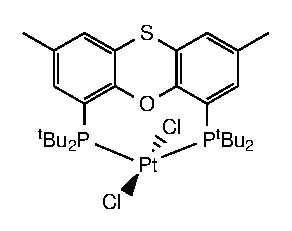
\includegraphics{../Structures/StBuPtCl2.eps}
%\end{center}
%\end{structure}

\tBuThixantphos{} (0.198 g, 0.38 mmol) and \ce{[Pt(C6H10)Cl2]} (0.133 g, 0.38 mmol) were dissolved in toluene (10 mL) and heated to 50 \degC{} for three days, resulting in an orange solution.  The solvent was removed \emph{in vacuo} and the resulting solid was dissolved in a minimum of dichloromethane.  Diethyl ether was added until a small amount of oily residue became evident.  The sample was cooled to -14 \degC, resulting the title compound as red crystals (0.199 g, 66\%).

\Phosphorusintro{C6D6}
\NMRPPt{32.9}{2700}
\Protonintro{500}{C6D6}
\NMRsinglet{7.11}{\StBucH},
\NMRsinglet{6.98}{\StBuaH},
\NMRsinglet{1.86}{\StBugH},
\NMRPH{1.71}{vt}{7.3}{PCC\emph{H}\sub{3}},
\NMRbsinglet{1.56}{PCC\emph{H}\sub{3}},
\Carbonintro{125}{C6D6}
\NMRPC{155.8}{vt}{6.3}{\emph{C}O},
\NMRsinglet{134.3}{PC(Ar)\emph{C}H},
\NMRPC{131.0}{vt}{3.4}{\emph{C}(Ar)\ce{CH3}},
\NMRsinglet{129.9}{SC\emph{C}C(\ce{CH3})},
\NMRcoupled{124.0}{vt}{18.5}{P\emph{C}(Ar)},
\NMRcoupled{124.5}{vt}{6.7}{\emph{C}S},
\NMRsinglet{20.3}{C(Ar)\emph{C}\ce{H3}},
\NMRPC{39.7}{vt}{11.6}{PC\emph{C}\ce{H3}},
\NMRPC{38.8}{vt}{11.1}{PC\emph{C}\ce{H3}},
\NMRPC{32.8}{vt}{3.9}{P\emph{C}\ce{CH3}},
\NMRbsinglet{30.2}{P\emph{C}\ce{CH3}},
HRMS calcd for \ce{C30H46OP2SClPt} [M-Cl]$^+$ \emph{m/z} = 745.2060; found = 745.2052.

%%%%%%%%
%PtSitBuCl2 %
%%%%%%%%
\subsection*{\trans{}-[Pt(\tBusixantphos)\ce{Cl2}]}
%\begin{structure}[h]
%\begin{center}
%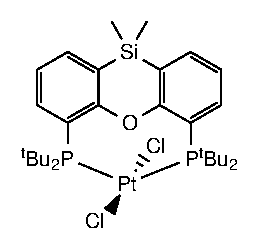
\includegraphics{../Structures/SitBuPtCl2.eps}
%\end{center}
%\end{structure}

A solution of \tBusixantphos{} (0.051 g, 0.10 mmol) in toluene (5 mL) was added to a suspension of \ce{[Pt(C6H10)Cl2]} (0.035 g, 0.10 mmol) in toluene (5 mL).  The reaction mixture was stirred at 50 \degC{} for 72 hours.  The solvent was removed under reduced pressure and the solid was taken up in \ce{C6D6} for NMR analysis.  The reaction showed a mixture of unreacted \tBusixantphos{} (53.4\%), \tBusixantphos \ce{H+} (22.8\%) and \trans-[Pt(\tBusixantphos)\ce{Cl2}] (23.8\%).  The NMR sample was heated at 50 \degC{} for a further 11 days.  At this stage no \ce{[Pt(C6H10)Cl2]} was observed in the \proton{} NMR spectrum and no change in the ratio of the compounds in the \phosphorus{} NMR spectrum was observed over a period of 24 hours.  The final ratio of the compounds was 63.8\% \tBusixantphos \ce{H+}, and 36.2\% \trans-[Pt(\tBusixantphos)\ce{Cl2}].  Attempts to isolate \trans-[Pt(\tBusixantphos)\ce{Cl2}] were unsuccessful.  Due to the complex nature of the \proton{} and \carbon{} NMR spectra for this system the product \trans-[Pt(\tBusixantphos)\ce{Cl2}] is proposed based on the similarities of the \phosphorus{} NMR spectrum with those for \trans-[Pt(\tButhixantphos)\ce{Cl2}] and \trans-[Pt(\tBuxantphos)\ce{Cl2}] which were formed \emph{via} the same reaction conditions. 

\begin{sloppypar}
\Phosphorusintro{C6D6}
\NMRPPt{34.7}{2686}.
HRMS calcd for \ce{C30H48ClOP2PtSi} [M-Cl\ce{]+} m/z = 739.2237; found = 739.2178.
\end{sloppypar}

%%%%%%%
%PtCtBuCl2%
%%%%%%%
\subsection*{Reaction of \tBuxantphos{} with [Pt(\ce{C6H10})\ce{Cl2}]}

%\begin{structure}[h]
%\begin{center}
%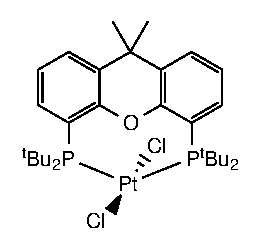
\includegraphics{../Structures/CtBuPtCl2.eps}
%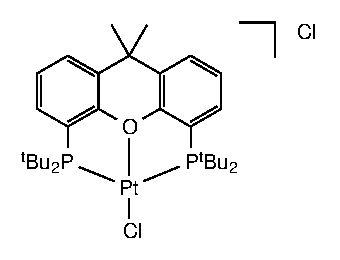
\includegraphics{../Structures/CtBuPtClCl.eps}
%\end{center}
%\end{structure}

A solution of \tBuxantphos{} (0.063 g, 0.126 mmol) in toluene (5 mL) was added to a suspension of \ce{[Pt(C6H10)Cl2]} (0.044 g, 0.126) in toluene (5 mL).  The reaction mixture was stirred at 50 \degC{} for 72 hours.  The solvent was removed \emph{in vacuo} leaving an orange solid.  The solid was recrystallised by inwards diffusion of diethyl ether into a dichloromethane solution of the complex, yielding the title complex as a yellow solid (0.027 g, 28\%).  The complex was analysed by NMR spectroscopy in \ce{C6D6}, \ce{CDCl3}, \ce{CD2Cl2} and \ce{d6-acetone}.  In \ce{C6D6} the complex is formulated as \trans-[Pt(\tBuxantphos)\ce{Cl2}] while in \ce{CDCl3} and \ce{CD2Cl2} the complex is thought to lose a chloride ligand resulting in [Pt(\tBuxantphosk)Cl]Cl.  In \ce{d6-acetone} the \phosphorus{} NMR spectrum appears as a broad singlet at 46 ppm.  The full NMR characterisation in the other solvents is given below.  

\subsubsection{\trans-[Pt(\tBuxantphos)\ce{Cl2}]}

\begin{sloppypar}
\Phosphorusintro{C6D6}
\NMRPPt{32.4}{2721.4}.
\Protonintro{500}{C6D6}
\NMRmultiplet{7.36}{\CtBucH},
\NMRcoupled{7.14}{d}{7.8}{\CtBuaH},
\NMRcoupled{6.89}{t}{7.0}{\CtBubH},
\NMRbsinglet{1.67}{\CtBujH},
\NMRsinglet{1.37}{\CtBuhH},
\NMRsinglet{1.40}{\CtBuhH}.
\Carbonintro{125}{C6D6}
\NMRcoupled{157.1}{vt}{6.3}{\CtBueC},
\NMRcoupled{136.0}{vt}{4.8}{\CtBufC},
\NMRsinglet{132.9}{\CtBucC},
\NMRsinglet{126.0}{\CtBuaC},
\NMRcoupled{122.5}{vt}{38.9}{\CtBudC},
\NMRcoupled{122.1}{vt}{6.3}{\CtBubC},
\NMRbsinglet{39.2}{\CtBuiC},
\NMRmultiplet{36.5}{\CtBuhC},
\NMRbsinglet{32.8}{\CtBujC},
\NMRsinglet{27.5}{\CtBuhC}.
\end{sloppypar}

\subsubsection{[Pt(\tBuxantphosk)Cl]Cl}

\begin{sloppypar}
\Phosphorusintro{CDCl3}
\NMRPPt{47.7}{2349.6}
\Protonintro{500}{CDCl3}
\NMRcoupled{7.96}{d}{7.9}{\CtBuaH},
\NMRbsinglet{7.93}{\CtBucH},
\NMRcoupled{7.70}{t}{7.3}{\CtBubH},
\NMRsinglet{1.80}{\CtBuhH},
\NMRPH{1.57}{vt}{15.6}{\CtBujH}.
\Carbonintro{125}{CDCl3}
\NMRPC{158.5}{vt}{11.0}{\CtBueC},
\NMRsinglet{134.7}{\CtBucC},
\NMRsinglet{133.8}{\CtBuaC},
\NMRsinglet{132.5}{\CtBufC},
\NMRPC{128.6}{vt}{6.8}{\CtBubC},
\NMRPC{117.2}{vt}{33.2}{\CtBudC},
\NMRPC{39.6}{vt}{21.1}{\CtBuiC},
\NMRsinglet{34.1}{\CtBuhC},
\NMRPC{30.1}{vt}{4.3}{\CtBujC},
\NMRsinglet{27.1}{\CtBugC}.
\end{sloppypar}

\Phosphorusintro{CD2Cl2}
\NMRPPt{47.8}{2345.3}
\Protonintro{500}{CD2Cl2}
\NMRmultiplet{7.93}{\CtBucH},
\NMRcoupled{7.78}{dd}{7.7, 1.2}{\CtBuaH},
\NMRcoupled{7.60}{t}{7.8}{\CtBubH},
\NMRsinglet{1.78}{\CtBuhH},
\NMRcoupled{1.57}{vt}{16.1}{\CtBujH}.
\Carbonintro{125}{CD2Cl2}
\NMRcoupled{158.8}{vt}{11.1}{\CtBueC},
\NMRsinglet{135.0}{\CtBucC},
\NMRsinglet{133.72}{\CtBuaC},
\NMRsinglet{132.7}{\CtBufC}
\NMRcoupled{128.3}{vt}{6.7}{\CtBubC},
\NMRcoupled{117.8}{vt}{33.1}{\CtBudC},
\NMRcoupled{39.8}{vt}{21.1}{\CtBuiC},
\NMRsinglet{34.5}{\CtBugC},
\NMRsinglet{34.1}{\CtBuhC},
\NMRcoupled{30.0}{vt}{4.8}{\CtBujC}.

HRMS calcd for \ce{C31H48ClOP2Pt} [M-Cl\ce{]+} m/z = 723.2468; found = 723.2455.

%%%%%%%%%
%PtStBuCl PF6%
%%%%%%%%%

\subsection*{[Pt(\tButhixantphosk)Cl]\ce{PF6}}

%\begin{structure}[h]
%\begin{center}
%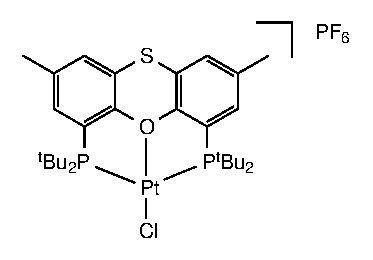
\includegraphics{../Structures/StBuPtClPF6.eps}
%\end{center}
%\end{structure}

Dissolved (\tBu-Thixantphos)platinum dichloride (0.035 g, 0.045 mmol) in dichloromethane (2 mL) and added ammonium hexafluorophosphate (0.015 g, 0.090 mmol).  After 1 hour of stirring the red solution had become yellow with a white precipitate.  The solution was filtered through a plug of alumina and the solvent removed \emph{in vacuo} yielding the title compound as a yellow solid (0.030g, 75\%).  

\Phosphorusintro{CD2Cl2}
\NMRPPt{46.4}{2347}
\NMRPF{-144.5}{septet}{710.5}{\emph{P}\ce{F6}}
\Protonintro{500}{CD2Cl2}
\NMRsinglet{7.41}{\StBucH},
\NMRsinglet{7.11}{\StBuaH},
\NMRsinglet{2.38}{\StBugH},
\NMRPH{1.55}{vt}{8.0}{\StBuiH},
\Carbonintro{125}{C6D6}
\NMRmultiplet{157.4}{\StBueC},
\NMRsinglet{138.9}{\StBubC},
\NMRsinglet{134.4}{\StBucC},
\NMRsinglet{132.6}{\StBuaC},
\NMRmultiplet{119.8}{\StBudC},
\NMRmultiplet{119.1}{\StBufC},
\NMRPC{40.0}{vt}{10.4}{\StBuhC},
\NMRsinglet{30.1}{\StBuiC},
\NMRsinglet{20.4}{\StBugC},
\Fluorineintro{CD2Cl2}
\NMRPF{-73.4}{d}{710.6}{P\emph{F}\sub{6}}
HRMS calcd for \ce{C30H46ClOP2PtS} [M-\ce{PF6]+} m/z = 741.2032; found = 741.2069.

%%%%%%%%%
% PtCtBuCl PF6 %
%%%%%%%%%

\subsection*{[Pt(\tBuxantphosk)Cl]\ce{PF6}}
%
%\begin{structure}[h]
%\begin{center}
%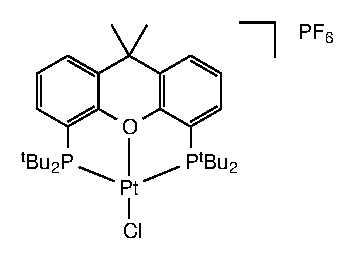
\includegraphics{../Structures/CtBuPtClPF6.eps}
%\end{center}
%\end{structure}

A solution of \tBuxantphos{} (0.014 g, 0.018 mmol) in dichloromethane (2.0 mL) was added to solid ammonium hexafluorophosphate (0.006 g, 0.037 mmol) in a Schlenk tube.  The reaction mixture was stirred for 1 hour before filtering through a plug of alumina.  The solvent was removed \emph{in vacuo} yielding the title compound as a yellow solid (0.008 g, 50\%).  

\sloppypar{}
\Phosphorusintro{CD2Cl2}
\NMRPPt{47.8}{2350.3},
-144.5 (septet, \JPF{} = 710.4 Hz, \ce{PF6}).
\Protonintro{600}{CD2Cl2}
\NMRmultiplet{7.92}{\CtBucH},
\NMRcoupled{7.82}{dd}{7.7, 1.5}{\CtBuaH},
\NMRcoupled{7.53}{t}{7.7}{\CtBubH},
\NMRsinglet{1.75}{\CtBuhH},
\NMRcoupled{1.57}{vt}{15.9}{\CtBujH}.
\Carbonintro{150}{CD2Cl2}
\NMRcoupled{158.8}{vt}{9.4}{\CtBueC},
\NMRsinglet{135.0}{\CtBucC},
\NMRsinglet{133.4}{\CtBuaC},
\NMRcoupled{132.6}{vt}{5.8}{\CtBufC},
\NMRcoupled{128.1}{vt}{6.4}{\CtBubC},
\NMRcoupled{118.0}{vt}{32.9}{\CtBudC},
\NMRcoupled{39.8}{vt}{21.4}{\CtBuiC},
\NMRsinglet{34.5}{\CtBugC},
\NMRsinglet{33.9}{\CtBuhC},
\NMRcoupled{30.0}{vt}{4.6}{\CtBujC}.
HRMS calcd for \ce{C31H48OP2Pt} [M-\ce{PF6}]$^+$ \emph{m/z} = 723.2468; found = 723.2513.

\subsection*{Attempted reaction of \tButhixantphos{} with [Pt(\ce{C6H10)Me2}]}

A solution of \tButhixantphos{} (0.020 g, 0.039 mmol) in \ce{C6D6} (0.5 mL) was added to an NMR tube containing [Pt(\ce{C6H10)Me2}].  No reaction was observed after 24 hours at room temperature.  The reaction was heated to 60 \degC{}.  After 28 days no conversion was evident by \phosphorus{} or \proton{} NMR spectroscopy.  \ce{CH2(SO2CF3)2} (1 eq.) was added, resulting in the immediate formation of [(\tButhixantphos)\ce{H]+}.

%%%%%%%%%
% PtStBuMe Cl %
%%%%%%%%%
\subsection*{[Pt(\tButhixantphosk)Me]Cl}

%\begin{structure}[h]
%\begin{center}
%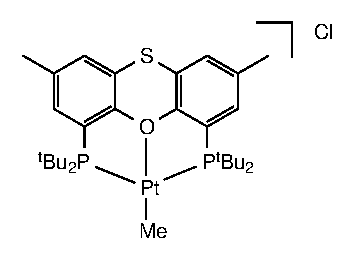
\includegraphics{../Structures/StBuPtMe.eps}
%\end{center}
%\end{structure}

A solution of \tButhixantphos{} (0.043 g, 0.083 mmol) in toluene (1.0 mL) was added to solid [Pt\ce{(C6H10)}ClMe] (0.027 g, 0.083 mmol) in a Schlenk tube.  The reaction mixture was stirred for 24 hours at room temperature, during which, an off-white precipitate formed.  The solution was decanted and the   solid dried under vacuum, giving [Pt(\tButhixantphos)Me]Cl as an off-white powder (0.057 g, 90\%).

\begin{sloppypar}
\Phosphorusintro{acetone-d6}
\NMRPPt{50.5}{2793.3}
\Protonintro{600}{acetone-d6}
\NMRPH{7.69}{d}{1.8}{\StBucH},
\NMRPH{7.34}{d}{1.2}{\StBuaH},
\NMRsinglet{2.42}{\StBugH},
\NMRPH{1.56}{vt}{15.6}{\StBuiH},
\NMRPH{1.94}{t}{5.5, \twoJPtH{}~=~97.4}{Pt-C\emph{H}\sub{3}},
\Carbonintro{150}{acetone-d6}
\NMRPC{153.8}{vt}{10.3}{\StBueC},
\NMRPC{137.1}{vt}{6.3}{\StBubC},
\NMRsinglet{134.4}{\StBucC},
\NMRsinglet{131.4}{\StBuaC},
\NMRPC{120.8}{vt}{31.8}{\StBudC},
\NMRPC{118.2}{vt}{7.2}{\StBufC},
\NMRPC{38.8}{vt}{20.6}{\StBuhC},
\NMRobscuredC{29.6}{HSQC}{\StBuiC},
\NMRsinglet{19.2}{\StBugC},
\NMRPC{-23.8}{t}{5.6, \oneJPtC{}~=~777.2}{Pt-\emph{C}\ce{H3}}
HRMS calcd for \ce{C31H49OP2PtS} [M-Cl]$^+$ \emph{m/z} = 721.2579; found = 721.2602.
\end{sloppypar}

%%%%%%%%%
% PtCtBuMe Cl %
%%%%%%%%%

\subsection*{[Pt(\tBuxantphos)Me]Cl}
%
%\begin{structure}[h]
%\begin{center}
%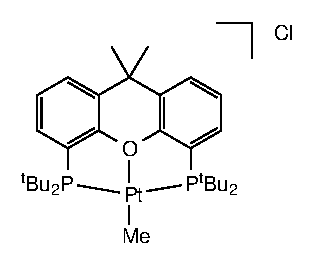
\includegraphics{../Structures/CtBuPtMe.eps}
%\end{center}
%\end{structure}

A solution of \tBuxantphos{} (0.024 g, 0.048 mmol) in toluene (0.5 mL) was added to solid [Pt\ce{(C6H10)}ClMe] (0.016 g, 0.048 mmol) in a Schlenk tube.  The reaction mixture was stirred for 24 hours at room temperature, during which, an off-white precipitate formed.  The solution was decanted and the   solid dried under vacuum, giving the title compound as an off-white powder (0.028 g, 78\%).

\Phosphorusintro{acetone-d6}
\NMRPPt{51.0}{2788.2}
\Protonintro{500}{acetone-d6}
\NMRcoupled{8.15}{dt}{7.5, 3.7}{\CtBucH},
\NMRcoupled{8.07}{d}{7.8}{\CtBuaH},
\NMRcoupled{7.63}{t}{7.9}{\CtBubH},
\NMRPH{1.92}{t}{5.4, \twoJPtH{}~=~97.4}{Pt-C\emph{H}\sub{3}},
\NMRsinglet{1.78}{\CtBuhH}
\NMRPH{1.55}{vt}{15.4}{\CtBujH}
\Carbonintro{125}{acetone-d6}
\NMRPC{156.1}{vt}{10.2}{\CtBueC},
\NMRsinglet{135.9}{\CtBucC},
\NMRsinglet{133.2}{\CtBuaC},
\NMRsinglet{132.7}{\CtBufC},
\NMRPC{127.4}{vt}{6.6}{\CtBubC},
\NMRPC{119.7}{vt}{34.1}{\CtBudC},
\NMRPC{39.5}{vt}{21.4, \twoJPtC{}~=~43.3}{\CtBuiC},
\NMRsinglet{35.0}{\CtBugC},
\NMRsinglet{33.7}{\CtBuhC},
\NMRPC{30.4}{vt}{6.1}{\CtBujC}.
\NMRPC{-23.9}{t}{5.6, \oneJPtC{}~=~774.6}{Pt-\emph{C}\ce{H3}}
HRMS calcd for \ce{C32H51OP2Pt} [M-Cl]$^+$ \emph{m/z} = 703.3014; found = 703.2987.


%%%%%%%%%
% PtSitBuMe Cl %
%%%%%%%%%

\subsection*{[Pt(\tBusixantphos)Me]Cl}

%\begin{structure}[h]
%\begin{center}
%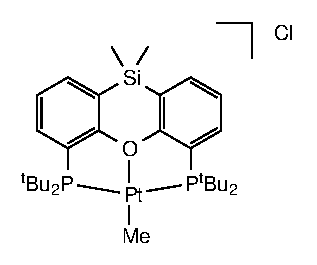
\includegraphics{../Structures/SitBuPtMe.eps}
%\end{center}
%\end{structure}

A solution of \tBusixantphos{} (0.026 g, 0.051 mmol) in \ce{C6D6} was added to an NMR tube containing [Pt\ce{(C6H10)}ClMe] (0.017 g, 0.051 mmol).  After 72 hours at room temperature little reaction was observed, so the solution was heated to 50\degC{} for 24 hours during which time a white precipitate formed.  NMR spectroscopy showed no unreacted \tBusixantphos{} was evident in the \proton{} or \phosphorus{} NMR spectra.  The solution was decanted and the title compound was dried under vacuum (0.014 g, 36\%).  

%Experiment 6006
\Phosphorusintro{acetone-d6}
\NMRPPt{48.7}{2762.9}
\Protonintro{500}{acetone-d6}
\NMRmultiplet{8.39-8.36}{\SitBucH},
\NMRdd{8.11}{7.1}{1.7}{\SitBuaH},
\NMRcoupled{7.65}{t}{7.4}{\SitBubH},
\NMRcoupled{2.01}{t}{5.5 \twoJPtH{}~=~98.6}{Pt-C\emph{H}\sub{3}},
\NMRcoupled{1.55}{vt}{15.2}{\SitBuiH},
\NMRsinglet{0.59}{\SitBugH}.
\Carbonintro{125}{acetone-d6}
\NMRPC{167.3}{vt}{8.2}{\SitBueC},
\NMRsinglet{140.72}{\SitBucC},
\NMRsinglet{140.67}{\SitBuaC},
\NMRPC{126.1}{vt}{6.1}{\SitBubC},
\NMRsinglet{123.5}{\SitBufC},
\NMRPC{121.2}{vt}{32.4}{\SitBudC},
\NMRPC{39.7}{vt}{21.8}{\SitBuhC},
\NMRPC{30.6}{vt}{5.6}{\SitBuiC},
\NMRsinglet{-0.5}{\SitBugC},
\NMRPC{-22.7}{t}{5.6, \oneJPtC{}~=~780.5}{Pt-\emph{C}\ce{H3}}.
HRMS calcd for \ce{C31H51OP2PtSi} [M-Cl]$^+$ \emph{m/z} = 724.2829; found = 724.2760.

\section{Palladium Complexes}
\label{section:experimental:palladium}

%%%%%%
% PdStBu%
%%%%%%
\subsection*{Reaction of \tButhixantphos{} with [Pd(nb\ce{)3}]}

A solution of \tButhixantphos{} (0.051 g, 0.10 mmol) in \ce{C6D6} (0.5 mL) was added to an NMR tube containing [Pd(nb\ce{)3}] (0.038 g, 0.10 mmol) and a small crystal of norbornene.  The NMR tube was sealed with a J. Young's tap.  After 72 hours at room temperature no \tButhixantphos{} was present by \phosphorus{} NMR spectroscopy.  The mixture contained [Pd(\tButhixantphos)] (62.0\%) and [Pd(\tButhixantphos)(nb)] (38.0\%).  

\subsubsection{[Pd(\tButhixantphos)(nb)]}

\Phosphorusintro{C6D6}
\NMRPsinglet{33.6}

\subsubsection{[Pd(\tButhixantphos)]}

%\begin{structure}[h]
%\begin{center}
%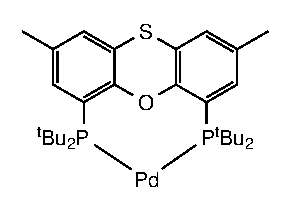
\includegraphics{../Structures/StBuPd14.eps}
%\end{center}
%\end{structure}

A solution of \tButhixantphos{} (0.056 g, 0.11 mmol) in toluene (1.0 mL) was added to a Schlenk tube containing [Pd(nb\ce{)3}] (0.042 g, 0.11 mmol) and a small crystal of norbornene (0.012 g).  The reaction was stirred overnight.  The solvent was removed \emph{in vacuo} leaving [Pd(\tButhixantphos)] as a oily brown solid (0.061 g, 90\%).

\Phosphorusintro{C6D6}
\NMRPsinglet{42.9}
\Protonintro{500}{C6D6}
\NMRsinglet{7.35}{\StBucH},
\NMRsinglet{6.83}{\StBuaH},
\NMRsinglet{1.95}{\StBugH},
\NMRPH{1.46}{vt}{13.7}{\StBuiH},
\Carbonintro{125}{C6D6}
\NMRPC{155.9}{vt}{14.0}{\StBueC},
\NMRsinglet{133.6}{\StBucC},
\NMRsinglet{131.9}{\StBubC},
\NMRsinglet{128.8}{\StBuaC}
\NMRPC{127.8}{vt}{8.2}{\StBudC},
\NMRPC{124.6}{vt}{5.3}{\StBufC},
\NMRPC{35.7}{vt}{3.8}{\StBuhC},
\NMRsinglet{31.9}{\StBuiC},
\NMRsinglet{20.4}{\StBugC}

\subsection*{Reaction of \tBuxantphos{} with [Pd(nb\ce{)3}]}

A solution of \tBuxantphos{} (0.046 g, 0.092 mmol) in \ce{C6D6} (0.5 mL) was added to an NMR tube containing [Pd(nb\ce{)3}] (0.036 g, 0.092 mmol) and a small crystal of norbornene.  The NMR tube was sealed with a J. Young's tap.  The NMR after one hour showed a mixture with no uncoordinated \tBuxantphos{} and multiplet products.  The mixture contained [Pd(\tBuxantphos)] (73.1\%) and [Pd(\tBuxantphos)(nb)] (12.6\%), as well as several other unidentified phosphorus containing compounds.  

\subsubsection*{[Pd(\tBuxantphos)(nb)]}

\Phosphorusintro{C6D6}
\NMRPsinglet{32.6}

\subsubsection*{[Pd(\tBuxantphos)]}

\Phosphorusintro{C6D6}
\NMRPsinglet{42.6}

\subsection*{[Pd(\tBusixantphos)]}

A solution of \tBusixantphos{} (0.040 g, 0.078 mmol) in \ce{C6D6} (0.5 mL) was added to a J. Young's tap NMR tube containing [Pd(nb\ce{))3}] (0.030 g, 0.078 mmol) and norbornene (0.010 g).  The tube was sealed under argon and the reaction was followed by NMR spectroscopy.  After 48 hours at room temperature a mixture of uncoordination \tBusixantphos{} (56.9\%) and [Pd(\tBusixantphos)] (43.1\%) is present by \phosphorus{} NMR.  After 24 hours no progress was observed.  However, after six months, the mixture contained \tBusixantphos{} (32.0\%) and [Pd(\tBusixantphos)] (68\%).  

\Phosphorusintro{C6D6}
\NMRPsinglet{41.9}
\Protonintro{300}{C6D6}
\NMRmultiplet{7.51}{\SitBucH},
\NMRcoupled{7.30}{dd}{7.1, 1.5}{\SitBuaC},
\NMRcoupled{6.92}{t}{7.4}{\SitBubC},
\NMRbsinglet{1.63}{\SitBuiH},
\NMRsinglet{0.23}{\SitBugH}.

\subsection*{[Pd(\tButhixantphos)(\hapto{2}-\ce{O2})]}

Air was bubbled through a solution of [Pd(\tButhixantphos)] (0.058 g, 0.093 mmol) in \ce{C6D6} (0.5 mL) for 10 minutes.  The solution turned green immediately.  The sample was filtered through a plug of alumina and reduced to dryness giving the title compound as a green solid (0.052 g, 90\%).

\Phosphorusintro{CDCl3}
\NMRPsinglet{52.0}
\Protonintro{500}{CDCl3}
\NMRsinglet{7.49}{2H, Ar},
\NMRsinglet{7.23}{2H, Ar},
\NMRsinglet{2.32}{\StBugH},
\NMRcoupled{1.50}{d}{13.7}{\StBuiH}.

%%%%%%%%
%PdCl2 SitBu %
%%%%%%%%
%\newpage{}
%2021
\subsection*{\trans{}-[Pd(\tBusixantphos)\ce{Cl2}]}

%\begin{structure}[h]
%\begin{center}
%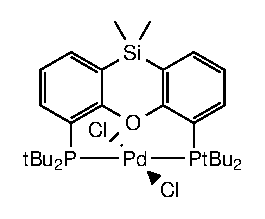
\includegraphics{../Structures/PdCl2(Si(tBu)2)_complex.eps}
%\end{center}
%\end{structure}

Combined \tBusixantphos{} (0.015 g, 0.029 mmol) and \ce{[Pd(cod)Cl2]} (0.008 g, 0.029 mmol) in an sealed tube and stirred at 60 \degC{} for hours then 35\degC{}.  The solvent was removed \emph{in vacuo} yielding the title compound as a red solid (0.018 g, 89\%).

\Phosphorusintro{CDCl3}
\NMRPsinglet{45.7}
\Protonintro{500}{CDCl3}
\NMRmultiplet{7.71}{\SitBucH},
\NMRHH{7.68}{d}{7.1}{\SitBuaH},
\NMRHH{7.33}{t}{7.3}{\SitBubH},
\NMRPH{1.60}{vt}{7.3}{\SitBuiH},
\NMRsinglet{0.52}{\SitBugH}.
\Carbonintro{125}{CDCl3}
\NMRPC{165.1}{vt}{6.8}{\SitBueC},
\NMRsinglet{137.6}{\SitBucC},
\NMRsinglet{136.9}{\SitBuaC},
\NMRsinglet{124.9}{\SitBufC},
\NMRsinglet{123.1}{\SitBubC},
\NMRPC{121.8}{vt}{13.4}{\SitBudC},
\NMRPC{39.6}{vt}{6.3}{\SitBuhC},
\NMRPC{31.1}{vt}{2.7}{\SitBuiC},
\NMRsinglet{-2.0}{\SitBugC}.

\Phosphorusintro{CD2Cl2}
\NMRPsinglet{46.7}
\Protonintro{600}{CD2Cl2}
\NMRmultiplet{7.72-7.74}{2H, \SitBuaH, \SitBucH},
\NMRcoupled{7.35}{t}{7.2}{\SitBubH},
\NMRcoupled{1.59}{vt}{15.0}{\SitBuiH},
\NMRsinglet{0.53}{\SitBugH}.
\Carbonintro{150}{CD2Cl2}
\NMRbsinglet{165.4}{\SitBueC},
\NMRsinglet{137.9}{\SitBucC},
\NMRsinglet{137.2}{\SitBuaC},
\NMRsinglet{125.2}{\SitBufC},
\NMRsinglet{123.2}{\SitBubC},
\NMRcoupled{122.0}{vt}{25.4}{\SitBudC},
\NMRcoupled{39.7}{vt}{12.8}{\SitBuhC},
\NMRbsinglet{31.1}{\SitBuiC},
\NMRsinglet{-2.2}{\SitBugC}.

\Phosphorusintro{C6D6}
\NMRPsinglet{42.0}
\Protonintro{500}{C6D6}
\NMRcoupled{7.51}{dtd}{7.7, 3.9, 1.8}{\SitBucH},
\NMRcoupled{7.30}{dd}{7.0, 1.6}{\SitBuaH},
\NMRcoupled{6.92}{t}{7.3}{\SitBubH},
\NMRbsinglet{1.64}{\SitBuiH},
\NMRsinglet{0.23}{\SitBugH}.
\Carbonintro{125}{C6D6}
\NMRcoupled{164.9}{vt}{6.2}{\SitBueC},
\NMRsinglet{137.2}{\SitBucC},
\NMRsinglet{135.5}{\SitBuaC},
\NMRcoupled{125.4}{vt}{3.0}{\SitBufC},
\NMRcoupled{124.1}{vt}{26.9}{\SitBudC},
\NMRcoupled{121.9}{vt}{4.8}{\SitBubC},
\NMRcoupled{39.4}{vt}{11.5}{\SitBuhC},
\NMRbsinglet{31.6}{\SitBuiC},
\NMRbsinglet{-3.1}{\SitBugC}.

HRMS calcd for \ce{C30H48OP2SiPdCl} [M-Cl]$^+$ \emph{m/z} = 655.1676; found = 655.1663.


%%%%%%%%
% PdStBuCl2 %
%%%%%%%%
\subsection*{\trans{}-[Pd(\tButhixantphos)\ce{Cl2}]}

%\begin{structure}[h]
%\begin{center}
%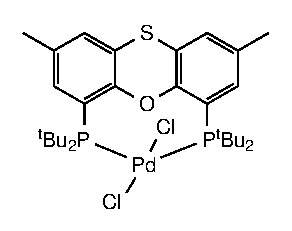
\includegraphics{../Structures/StBuPdCl2.eps}
%\end{center}
%\end{structure}

\tBuThixantphos{} (0.197 g, 0.38 mmol) and \ce{[Pd(cod)Cl2]} (0.108 g, 0.38 mmol) were dissolved in toluene then heated to 40\degC{} for three days.  The solvent was removed \emph{in vacuo} yielding the title compound as an orange solid (0.265 g, 100\%).


%2020%
%\Phosphorusintro{CD2Cl2}
%\NMRPsinglet{41.9}
%\Protonintro{500}{CD2Cl2}
%\NMRsinglet{7.17}{\StBucH},
%\NMRsinglet{7.15}{\StBuaH},
%\NMRsinglet{2.33}{\StBugH},
%\NMRPH{1.59}{vt}{7.1}{\StBuiH}.
%\Carbonintro{125}{C6D6}
%\NMRPC{155.1}{vt}{4.8}{\StBueC},
%\NMRsinglet{134.4}{\StBucC},
%\NMRPC{133.4}{vt}{\StBubC},
%\NMRsinglet{130.4}{\StBuaC},
%\NMRPC{123.5}{vt}{12.5}{\StBudC},
%\NMRsinglet{123.1}{\StBufC},
%\NMRPC{39.5}{vt}{5.8}{\StBuhC},
%\NMRsinglet{31.2}{\StBuiC},
%\NMRsinglet{20.7}{\StBugC}.

%7032%
\Phosphorusintro{CD2Cl2}
\NMRPsinglet{40.0}
\Protonintro{600}{CD2Cl2}
\NMRsinglet{7.16}{\StBuaH},
\NMRsinglet{7.15}{\StBucH},
\NMRsinglet{2.33}{\StBugH},
\NMRcoupled{1.59}{vt}{13.6}{\StBuiH},
\Carbonintro{150}{CD2Cl2}
\NMRcoupled{155.1}{vt}{8.7}{\StBueC},
\NMRsinglet{134.4}{\StBuaC},
\NMRcoupled{133.1}{vt}{5.8}{\StBubC},
\NMRsinglet{130.2}{\StBucC},
\NMRcoupled{123.8}{vt}{26.1}{\StBudC},
\NMRcoupled{123.3}{vt}{6.3}{\StBufC},
\NMRcoupled{39.5}{vt}{12.1}{\StBuhC},
\NMRbsinglet{31.3}{\StBuiC},
\NMRsinglet{20.7}{\StBugC}.
HRMS calcd for \ce{C30H46OP2SPdCl} [M-Cl]$^+$ \emph{m/z} = 657.1468; found = 657.1446.

%%%%%%%%
% PdCtBuCl2%
%%%%%%%%

\subsection*{\trans{}-[Pd(\tBuxantphos)\ce{Cl2}]}

\tBuXantphos{} (0.021 g, 0.042 mmol) and \ce{[Pd(cod)Cl2]} (0.012 g, 0.042 mmol) were dissolved in \ce{C6D6} in an NMR tube then heated to 40\degC{} for three days.  The solvent was removed \emph{in vacuo} and the residue was washed with pentane yielding the title compound as an orange solid (0.015 g, 53\%).

%\begin{structure}[h]
%\begin{center}
%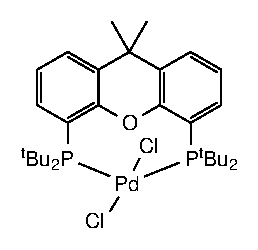
\includegraphics{../Structures/CtBuPdCl2.eps}
%\end{center}
%\end{structure}

\begin{sloppypar}
\Phosphorusintro{C6D6}
\NMRPsinglet{40.0}
\Protonintro{600}{C6D6}
\NMRcoupled{7.33}{dtd}{8.1, 3.4, 1.5}{\CtBucH},
\NMRcoupled{7.13}{dd}{7.7, 1.2}{\CtBuaH},
\NMRcoupled{6.87}{t}{7.7}{\CtBubH},
\NMRbsinglet{1.65}{\CtBujH},
\NMRbsinglet{1.32}{\CtBuhH}.
\Carbonintro{150}{C6D6}
\NMRcoupled{156.9}{vt}{8.7}{\CtBueC},
\NMRcoupled{135.4}{vt}{4.6}{\CtBufC},
\NMRsinglet{132.8}{\CtBucC},
\NMRsinglet{126.2}{\CtBuaC},
\NMRcoupled{123.0}{vt}{27.7}{\CtBudC},
\NMRcoupled{122.2}{vt}{5.3}{\CtBubC},
\NMRcoupled{39.1}{vt}{12.1}{\CtBuiC},
\NMRsinglet{36.2}{\CtBugC},
\NMRbsinglet{31.5}{\CtBujC},
\NMRsinglet{24.9}{\CtBuhC}.
\end{sloppypar}

\begin{sloppypar}
\Phosphorusintro{CD2Cl2}
\NMRPsinglet{54.1}
\Protonintro{600}{CD2Cl2}
\NMRcoupled{7.87}{d}{7.6}{\CtBuaH},
\NMRmultiplet{7.76}{\CtBucH},
\NMRcoupled{7.52}{t}{7.7}{\CtBubH},
\NMRsinglet{1.75}{\CtBuhC},
\NMRcoupled{1.59}{vt}{15.5}{\CtBujH},
\Carbonintro{150}{CD2Cl2}
\NMRcoupled{156.6}{vt}{11.6}{\CtBueC},
\NMRsinglet{134.6}{\CtBufC}
\NMRsinglet{132.0}{\CtBucC},
\NMRsinglet{126.5}{\CtBuaC},
\NMRcoupled{118.1}{vt}{24.3}{\CtBudC},
\NMRsinglet{117.6}{\CtBubC},
\NMRcoupled{39.8}{vt}{13.8}{\CtBuiC},
\NMRsinglet{32.6}{\CtBugC},
\NMRsinglet{31.4}{\CtBuhC},
\NMRcoupled{30.3}{vt}{5.8}{\CtBujC}.
\end{sloppypar}

HRMS calcd for \ce{C31H48OP2PdCl} [M-Cl]$^+$ \emph{m/z} = 635.1925; found = 635.1966.


%%%%%%%%%%
% PdStBuCl PF6 %
%%%%%%%%%%
\subsection*{[Pd(\tButhixantphosk)Cl]\ce{PF6}}

%\begin{structure}[h]
%\begin{center}
%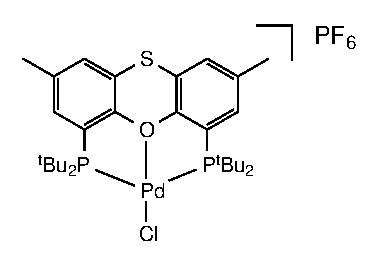
\includegraphics{../Structures/StBuPdClPF6.eps}
%\end{center}
%\end{structure}

\ce{NH4PF6} (0.052 g, 0.32 mmol) and \trans-[Pd(\tButhixantphos)\ce{Cl2}] (0.050, 0.061 mmol) were combined in an Schlenk tube and suspended in \ce{CH2Cl2} (10 mL).  The reaction mixture was stirred overnight and the volume was reduced by half.  The solution was filtered through a plug of alumina and reduced to dryness giving the title compound as a yellow solid (0.039 g, 68\%).  

\Phosphorusintro{CD2Cl2}
\NMRPsinglet{56.4}
\NMRPF{-144.5}{septet}{710.5}{\emph{P}\ce{F6}}
\Protonintro{500}{CD2Cl2}
\NMRPH{7.36}{d}{2.0}{\StBucH},
\NMRsinglet{7.15}{\StBuaH},
\NMRsinglet{2.38}{\StBugH},
\NMRPH{1.58}{vt}{8.2}{\StBuiH},
\Carbonintro{125}{C6D6}
\NMRPC{154.86}{vt}{6.5}{\StBueC},
\NMRPC{138.3}{vt}{5.8}{\StBubC},
\NMRsinglet{134.6}{\StBucC},
\NMRsinglet{132.6}{\StBuaC},
\NMRsinglet{119.1}{\StBufC},
\NMRPC{118.7}{vt}{10.8}{\StBudC},
\NMRPC{40.2}{vt}{7.2}{\StBuhC},
\NMRsinglet{30.1}{\StBuiC},
\NMRsinglet{20.4}{\StBugC}
\Fluorineintro{CD2Cl2}
\NMRPF{-73.4}{d}{710.6}{P\emph{F}\sub{6}}
HRMS calcd for \ce{C30H46ClOP2PdS} [M-\ce{PF6]+} m/z = 653.1489; found = 653.1527.

%%%%%%%%%%
% PdSitBuCl PF6 %
%%%%%%%%%%

\subsection*{[Pd(\tBusixantphosk)Cl]\ce{PF6}}

%\begin{structure}[h]
%\begin{center}
%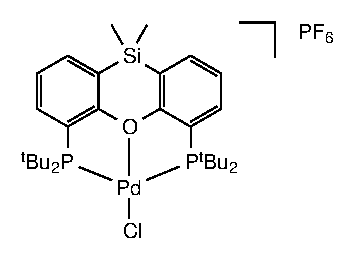
\includegraphics{../Structures/SitBuPdClPF6.eps}
%\end{center}
%\end{structure}

This compound was synthesised as for [Pd(\tButhixantphosk)Cl]\ce{PF6} using \trans{}-[Pd(\tBusixantphos)\ce{Cl2}] (0.018 g, 0.026 mmol) and \ce{NH4PF6} (0.005 g, 0.030 mmol) giving the title compound as a yellow solid (0.020 g, 96\%).

\begin{sloppypar}
\Phosphorusintro{CD2Cl2}
\NMRPasysinglet{52.4}{\tBusixantphos}
\NMRPF{-144.5}{septet}{710.3}{\ce{PF6}}
\Protonintro{500}{CD2Cl2}
\NMRmultiplet{8.07}{\SitBucH},
\NMRcoupled{7.91}{dd}{7.0, 1/9}{\SitBuaH},
\NMRcoupled{7.56}{t}{7.4}{\SitBubH},
\NMRcoupled{1.59}{vt}{16.1}{\SitBuiH},
\NMRsinglet{0.60}{\SitBugH}.
\Carbonintro{125}{CD2Cl2}
\NMRcoupled{168.4}{vt}{10.6}{\SitBueC},
\NMRsinglet{140.9}{\SitBuaC},
\NMRsinglet{139.7}{\SitBucC},
\NMRcoupled{126.1}{vt}{5.3}{\SitBubC},
\NMRsinglet{124.1}{\SitBufC}
\NMRcoupled{118.0}{vt}{22.1}{\SitBudC},
\NMRcoupled{40.2}{vt}{15.4}{\SitBuhC},
\NMRcoupled{30.2}{vt}{5.3}{\SitBuiC},
\NMRsinglet{-0.4}{\SitBugC}.
\Fluorineintro{CD2Cl2}
\NMRcoupled{-73.4}{d}{-706.6}{\ce{PF6}}
HRMS calcd for \ce{C30H48ClOP2PdSi} [M-\ce{PF6]+} m/z = 651.1694; found = 651.1717.
\end{sloppypar}

%%%%%%%%%%
% PdCtBuCl PF6 %
%%%%%%%%%%
\subsection*{[Pd(\tBuxantphosk)Cl]\ce{PF6}}

%\begin{structure}[h]
%\begin{center}
%\includegraphics{../Structures/CtBuPdClPF6.eps}
%\end{center}
%\end{structure}

This compound was synthesised as for [Pd(\tButhixantphosk)Cl]\ce{PF6} using \trans{}-[Pd(\tBuxantphos)\ce{Cl2}] (0.020 g, 0.030 mmol) and \ce{NH4PF6} (0.005 g, 0.030 mmol) giving the title compound as a yellow solid (0.020 g, 86\%).

\begin{sloppypar}
\Phosphorusintro{CD2Cl2}
\NMRPasysinglet{58.3}{\tBuxantphos},
\NMRPF{-144.5}{septet}{710.4}{\ce{PF6}}
\Protonintro{500}{CD2Cl2}
\NMRcoupled{7.87}{dd}{7.7, 1.6}{\CtBucH},
\NMRmultiplet{7.84}{\CtBuaH},
\NMRcoupled{7.53}{t}{7.9}{\CtBubH},
\NMRsinglet{1.76}{\CtBuhH},
\NMRcoupled{1.59}{vt}{16.1}{\CtBuhH}
\Carbonintro{125}{CD2Cl2}
\NMRcoupled{156.7}{vt}{11.6}{\CtBueC},
\NMRsinglet{135.1}{\CtBucC},
\NMRsinglet{133.4}{\CtBuaC},
\NMRbsinglet{132.7}{\CtBufC},
\NMRcoupled{127.4}{vt}{6.6}{\CtBubC},
\NMRcoupled{117.1}{vt}{24.0}{\CtBudC},
\NMRcoupled{40.1}{vt}{14.9}{\CtBuiC},
\NMRsinglet{34.5}{\CtBugC},
\NMRsinglet{34.0}{\CtBuhC},
\NMRcoupled{30.0}{vt}{7.3}{\CtBujC}.
\Fluorineintro{CD2Cl2}
\NMRcoupled{-73.5}{d}{-709.6}{\ce{PF6}}
HRMS calcd for \ce{C31H48ClOP2Pd} [M-\ce{PF6]+} m/z = 635.1925; found = 635.1959.
\end{sloppypar}

%%%%%%%%%%%%
%% PdOAc2 + SitBu %
%%%%%%%%%%%%
%\subsection*{Reaction of \tBusixantphos{} and palladium acetate}
%
%%7003%
%A solution of \tBusixantphos{} (0.034 g, 0.066 mmol) in \fixme{d6-benzene} (0.5 mL) was added to solid \ce{[Pd(OAc)2]} in a glass tube.  The tube was sealed with a septum and heated to 60 \degC for a total of 24 hours.  However, no change was observed after the first four hours.  The solvent was removed in vacuo yielding a dark red solid (0.034 g) which was analysed by ATR-IR in dichloromethane and mass spectrometry.  
%
%%%%%%%%%%
%% PdStBuOAc2 %
%%%%%%%%%%
%\subsection*{\emph{trans}-(\emph{t}-Bu-Thixantphos)palladiumdiacetate}
%
%\begin{structure}[h]
%\begin{center}
%\includegraphics{../Structures/StBuPdOAc2.eps}
%\end{center}
%\end{structure}
%
%\Phosphorusintro{C6D6}
%\NMRPsinglet{33.7}
%\Protonintro{500}{C6D6}
%\NMRPH{7.07}{d}{2.0}{\StBucH},
%\NMRsinglet{6.83}{\StBuaH},
%\NMRsinglet{1.89}{\StBugH},
%\NMRbsinglet{1.42}{\StBuiH},
%\fixme{Peak for acetates?}
%\Carbonintro{125}{C6D6}
%\NMRbsinglet{177.7}{O\emph{C}(O)\ce{CH3}}
%\NMRPC{156.3}{vt}{8.4}{\StBueC},
%\NMRPC{134.4}{d}{13.9}{\StBucC},
%\NMRsinglet{132.9}{\StBubC},
%\NMRsinglet{129.9}{\StBuaC},
%\NMRPC{123.5}{vt}{\StBufC},
%\NMRPC{120.3}{vt}{22.4}{\StBudC},
%\NMRPC{37.0}{vt}{10.2}{\StBuhC},
%\NMRbsinglet{30.3}{\StBuiC},
%\NMRbsinglet{24.3}{OC(O)\emph{C}\ce{H3}}
%\NMRsinglet{20.3}{\StBugC}
%HRMS calcd for \ce{C30H46OP2PdS} [M-2(OAc)+Cl]$^+$ \emph{m/z} = 653.1489; found = 653.1507.
%
%\fixme{IR, EA, MS}




%\section{Lab work that would be nice to do}
%\begin{itemize}
%\item{VT NMR with the lithiated ligand to try and get P-Li coupling constant}
%\item{React 14-electron complex with silane and HCl to try and identify the unknown hydride that forms when reacting with Pt(COD)2 or Pt(nb)3}
%\item{Palladium analogue of PtMe}
%\item{Protonation of PtMe complex}
%\end{itemize}
%
%\section{Desk work that still needs to be done}
%\begin{itemize}
%\item{Complete bite-angle calculations}
%\item{Look up structures for Pt(P)2 on scifinder and CCD}
%	\begin{itemize}
%	\item{Check if there are any with diphosphines, van Leeuwens review suggested that there were not, there appear to be some for palladium Schnetz2008, Gold (Partyka2010, Dalton. Escalle2009, Inorg. Chem. Deschamps2006, Dalton, Gualco2012 Organometallics, Joost 2013, Organometallics, Siemeling2011, Z. Anorg. Allg. Chem., Mezilles1999, Angew, Sircoglou2008 Organometallics, Nasser2010, Chem. Comm., Bauer2010, Chem-Eur. J. Gibson1996, Dalton), Rhodium (Kim2004, Inorganic Chemistry), Silver (Harrington200, Polyhedron, Heuer2000, Polyhedron, Chikkali2007, Camalli1988, Helv., Meng2013, Polyhedron, Gualco2011, JACS)}
%	\end{itemize}
%\item{Check 600 MHz for a carbon on 4019 after 18/4}
%\item{Check solubility of CO across different temperatures}
%\item{Look at 4027 (oxidation of StBu) to try and find evidence of S oxidation}
%\item{Look at VT on 4029 - dichloride complex}
%\item{Fully assign 4031 (CtBu selenide?)}
%\item{Assign IR stretches}
%	\begin{itemize}
%	\item{It may be necessary to compare with calculated IRs}
%	\end{itemize}
%\item{Check the integrals for nb, ethene and COD complexes to go into thesis}
%\item{Update the synthesis books}
%\item{Read up on iridium hydride metallation stuff, see Kranenburg1995 for an unusual Rh complex}
%\item{Read Mora2008 to get ideas for catalysis}
%\item{Get mestranova NMR stuff for the VT on the dichloride (4009?) that I did}
%\end{itemize}

%\subsection*{2,4-Di(carbomethoxy)-1,5-bis(\emph{p}-dimethylaminophenyl)-penta-1,4-dien-3-one}

%\begin{structure}
%\begin{center}
%\includegraphics[scale=1.2]{structures/dba436}
%\end{center}
%\end{structure}


%\noindent Dimethyl 1,3-acetonedicarboxylate (3.5~g, 0.02 mol), \textit{p}-di\-methy\-lamino\-benz\-aldehyde (6.0~g, 0.04 mol), piperidine (0.45~\cm, 4.6~mmol) and glacial acetic acid (0.30~\cm, 5.2~mmol) were combined in benzene (60~\cm) in a 250~\cm{} round bottom flask in the air.  The flask was equipped with a Dean-Stark trap to measure the volume of water being eliminated during the course of the reaction.  The trap was in turn equipped with a condenser, and the reaction mixture was heated under reflux for 1 day.  About 0.7~\cm{} of water were collected in the Dean-Stark trap indicating that the reaction was complete.  The solvent was removed \textit{in vacuo} to yield a dark red oil.  The oil was washed with petroleum ether several times then taken up in benzene.  The mixture was stirred at room temperature for several hours during which yellow crystalline solid precipitated out as the oil slowly dissolved.  The solid was filtered, washed with benzene and dried in the air
%(7.5~g, 86\%); 
%mp 124.5-124.8\degC{} (from benzene);
%(Found: C, 69.2; H, 6.5; N, 6.4. \ce{C25H28N2O5} requires C, 68.8; H, 6.5; N, 6.4\%);
%\numax(KBr)/\percm{} 1732, 1719, 1701, 1693, 1572, 1526, 1373, 1189 and 1158;  
%\dH(300~MHz; \ce{C6D6}; \ce{Me4Si}) 
%2.18 (6 H, s, \ce{NMe2}), 
%2.19 (6 H, s, \ce{NMe2}), 
%3.43 (3 H, s, OMe), 
%3.69 (3 H, s, OMe), 
%6.12 (2 H, d, \JHH{} 9.0, \textit{m}-H), 
%6.23 (2 H, d, \JHH{} 9.0, \textit{m}-H), 
%7.31 (2 H, d, \JHH{} 9.0, \textit{o}-H), 
%7.62 (2 H, d, \JHH{} 9.0, \textit{o}-H), 
%7.88 (1 H, s, CH=CH) and 
%8.32 (1 H, s, CH=CH);  
%\dC(75~MHz; \ce{C6D6}; \ce{Me4Si}) 
%39.15 (2 C, s, \ce{NMe2}), 
%39.17 (2 C, s, \ce{NMe2}), 
%51.8 (1 C, s, OMe), 
%52.0 (1 C, s, OMe), 
%111.8 (1 C, s, \textit{m}-\ce{C6H4}), 
%112.1 (1 C, s, \textit{m}-\ce{C6H4}), 
%120.9 (2 C, s, \ce{C6H4}), 
%121.2 (2 C, s, \ce{C6H4}), 
%132.5 (2 C, s, \textit{o}-\ce{C6H4}), 
%133.2 (2 C, s, \textit{o}-\ce{C6H4}), 
%143.7 (1 C, s, \textit{p}-\ce{C6H4}), 
%143.9 (1 C, s, \textit{p}-\ce{C6H4}), 
%166.5 (1 C, s, COO), 
%169.3 (1 C, s, COO) and 
%193.8 (1 C, s, CO);
%\textit{m/z} (ESI) 459.1000 (\MplusNa. \ce{C25H28N2O5Na} requires 459.1896).